\documentclass[a5paper]{scrartcl}
\usepackage{riley}
\usepackage{riley-libertine}

\def\book#1{\textit{#1}}

\SetProtrusion[load=default]{font=*}{%
      {„}={1000,1000},
      {‟}={1000,1000},
  {.}={,1000}, {,}={,1000}, {-} = {,1000} , {;}={,900}, {:}={,900}, {?}={,400}, {\textquotedblleft} = {900,900}, {\textquotedblright}={900,900}, {\textquoteleft} = {1000,},{\textquoteright}={,1000} }


\usepackage{biblatex}
\addbibresource{bib.bib}
\setcounter{biburllcpenalty}{1000}
%https://tex.stackexchange.com/questions/494540/format-links-text-in-the-bibliography-to-be-exactly-like-other-links
\appto{\bibsetup}{\urlstyle{tt}}

\usepackage{tikz}
\usetikzlibrary{cd, arrows.meta, decorations.pathmorphing }

\let\oldamp\&
%\def\&{\textit{\oldamp}}

\def\cat{\mathcal{C}}
\def\dee{\mathcal{D}}
\def\topcat{\texttt{top}}
\def\setcat{\texttt{set}}
\def\grp{\texttt{grp}}
\def\veccat{\texttt{vec}}
\def\ab{\texttt{ab}}
\def\smooth{\texttt{smooth}}
\def\vecbundle{\texttt{vecBundle}}
\def\catcat{\texttt{cat}}
\def\cobord{\texttt{cobord}}


%\newcommand{\PI}{\mathbin{\text{\rotatebox[origin=c]{180}{\(\amalg\)}}}}
%https://tex.stackexchange.com/a/126173/16161
\newcommand{\PI}{\mathbin{\Pi}}

\let\oldbullet\bullet
\def\bullet{\color{gray}\oldbullet}

\newcommand{\obj}{\texttt{Ob}}
\newcommand{\arr}{\texttt{Ar}}

\newcommand{\gray}[1]{{\color{gray}#1}}
\newcommand{\black}[1]{{\color{black}#1}}

\newcommand{\gparen}[1]{\left .\!{\gray{\paren{\black{#1}}}}\!\right.}

\newcommand{\op}{\textrm{op}}
\newcommand{\marginnote}[1]{\normalmarginpar\marginpar{\tiny\sffamily\raggedright #1}}
\newcommand{\revmarginnote}[1]{\reversemarginpar\marginpar{\tiny\sffamily\raggedleft #1}}

\DeclareMathOperator{\floor}{\texttt{floor}}
\DeclareMathOperator{\ceil}{\texttt{ceil}}
\DeclareMathOperator*{\free}{\texttt{free}}
\DeclareMathOperator*{\forget}{\texttt{forget}}
\DeclareMathOperator*{\under}{\texttt{under}}

\DeclareMathOperator{\rat}{\texttt{Rational}}
\DeclareMathOperator*{\Hom}{hom}
\def\hom{\Hom}

\title{\normalfont \color{darkgray}Categories for a few specific working physicists}
\author{Riley Levy}


\let\oldimplies\implies
\def\implies{\color{gray}\oldimplies\color{black}}

\begin{document}
\maketitle
\section{Intro \& motivation}
Theoretical mathematics is, to first order of approximation, the study of objects with a \emph{structure} and the functions that \emph{preserve} this structure, its arrows/morphisms. The prototypical example is the vector space and linear maps. The story of vector spaces is told through linear maps. This is true in general. Here's a list of structures and their associated morphisms, which we'll soon call categories.
\begin{itemize}
  \item Sets \& functions (\setcat)
  \item Vector spaces \& linear functions (\veccat)
  \item Inner product spaces \& unitary functions
  \item Metric spaces \& isometries
  \item Groups \& homomorphsims
  \item Ordered sets \& order-preserving (non-decreasing) functions
  \item Topological spaces \& continuous functions (\topcat)
  \item Smooth Manifolds \& smooth functions (\smooth)
  \item Types \& computable functions
\end{itemize}

Before formalizing this, I want to mention some motivation. First, because familiar objects usually have multiple structures on them, it's important to specify which one we are interested in. As sets \(\R\) and \(\R^2\) have the same structure because they're bijective, but as vector spaces, they are different because they have different dimensions. We also want to recognize when seemingly-different objects actually have the same structure. Looking for structure-preserving invertible functions provides a general way to do this.

Formalizing this idea is the genesis of category theory.
\begin{defn}[Category]
  A category is a class\revmarginnote{They're often too big to be sets, but I won't discuss this today.} of objects \& a class of arrows between them.  Additionally, each object has an identity arrow, and the set of arrows are closed under composition.

  If \(\cat\) is a category, call its set of objects \(\obj(\cat)\). If \(A, B \in \obj(\cat)\), the set of arrows \(A\to B\), called the hom-set, is denoted\marginnote{Arrows are also called homomorphisms, especially in algebra.}
  \[
    \Hom_\cat(A,B).
  \]
  If \(f\in \Hom_\cat{A,B}\) and \(g\in \Hom_\cat(B,C)\), then
  \[
    g\circ f \in \Hom_\cat(A,C).
  \]
  so the following diagram \emph{commutes} (following any path shown between two objects gives the same answer)
  \[
    \begin{tikzcd}
      A\ar[bend right=3em,swap,"g\circ f"]{rr}\rar{f} & B\rar{g} & C
    \end{tikzcd}
  \]
  And identity arrows have the property
  \[
    f\circ 1_A = f \qquad 1_B \circ f = f
  \]
  \[
    \begin{tikzcd}
      A\arrow[loop left]{1_A}\rar{f}& B
    \end{tikzcd}
    \qquad
    \begin{tikzcd}
      A\rar{f}& B\arrow[loop right]{1_B}
    \end{tikzcd}
  \]
  for \(1_A \in \Hom(A,A)\) and \(1_B \in \Hom(B,B)\)
\end{defn}

\begin{lemma}[Identities are unique]
  Suppose \(I\) is an identity on \(A\). Then \(I = 1_A\).
\end{lemma}
\begin{proof}
  \[1_A = I \circ 1_A = I. \]
\end{proof}

\begin{defn}[Invertible]
  An arrow \(f: X \to Y\) is invertible, aka an isomorphism, iff there is some \(g: Y \to X\) such that
  \[
    1_X = g \circ f \qquad\text{and}\qquad 1_Y = f \circ g
  \]
  \ie, the following diagram \emph{commutes}:
  \[
    \begin{tikzcd}
      X\arrow[loop left,"1_X"]{}\rar[shift left =.2em]{f} & Y \arrow[loop right,"1_Y"]{} \lar[shift left=.2em]{g}
    \end{tikzcd}
  \]
\end{defn}
\begin{lemma}[Inverses are unique]
  If\eit/ \(L\) and\eit/ \(R\) are both inverses of\eit/ \(f\), then\eit/ \(L=R\).
\end{lemma}
\begin{proof}
\revmarginnote{Actually proves if there's both a left and right inverse, they are equal \& two-sided.}
  \[
    L = L \circ 1_B = L \circ \gparen{f \circ R} = \gparen{L\circ f}\circ R = 1_A \circ R = R
  \]
\end{proof}
One-sided inverses need not be unique, for example, a projection has multiple sections.

Groups theory axiomatizes the algebra of symmetry transformations. Category theory generalizes this by axiomatizing the algebra of all structure-preserving functions.
\begin{quote}
  ``This may be regarded as a continuation of the Klein Erlanger Programm, in the sense that a geometrical space with its group of transformations is generalized to a category with its algebra of mappings'' \cite[237]{natural-equivalence} (the founding paper)
\end{quote}

Our original motivation for arrows were functions, but it's useful to consider other possibilities.

\begin{defn}[The category of a partially-ordered set]
  If \((P,\leq)\) is a partially-ordered set, turn it into a category by drawing exactly one arrow \(x \to y\) iff \(x\leq y\).

  Existence of identity arrows comes from reflexivity, and existence of compositions comes from transitivity.
\end{defn}
For example, \(2^{\set{0,1,2}}\), the powerset of \(\set{0,1,2}\), is partially ordered by \(\subseteq\), so it forms the category
\[
  \begin{tikzcd}
    &\set{0,1,2} \arrow[loop left,gray]{} \\
    \set{0,1}\ar{ur}\arrow[loop left,gray]{} & \set{0,2}\ar{u} \arrow[loop left,gray]{} & \set{1,2}\ar{ul}\arrow[loop left,gray]{}  \\
    \set{0}\ar{u}\ar{ru}\ar[gray]{uur}\arrow[loop left,gray]{}  & \set{1}\ar{lu}\ar{ru}\ar[gray]{uu} \arrow[loop left,gray]{} &\set{2}\ar{ul}\ar{u}\ar[gray]{uul} \arrow[loop left,gray]{} \\
    & \emptyset\ar{lu}\ar{u}\ar[ru]\ar[gray]{uuu}\arrow[loop left,gray]{}
  \end{tikzcd}.
\]
This is usually drawn with identities and compositions omitted:
\[
  \begin{tikzcd}
    &\set{0,1,2} \\
    \set{0,1}\ar{ur}& \set{0,2}\ar{u} & \set{1,2}\ar{ul} \\
    \set{0}\ar{u}\ar{ru}& \set{1}\ar{lu}\ar{ur}&\set{2}\ar{ul}\ar{u}\\
    & \emptyset\ar{lu}\ar{u}\ar{ur}
  \end{tikzcd}
\]
In this way, category theory generalizes order theory. Many constructions in category theory correspond to familiar constructions in order theory, like \(\max\) and \(\sup\).

\begin{defn}[Proof-arrow category.]
  The objects are statements and each arrow \(A\to B\) is a proof of \(B\) given \(A\).

  Identity arrows exist because given \(a\) conclude \(a\) is a tautology, and compositions exist because proofs are transitive (the cut-elimination theorem).
\end{defn}

\begin{defn}[Path-arrow category]
  The objects are points in a topological space, and the arrows \(x\to y\) are paths from \(x\) to \(y\). Identities are the constant path, and composition is path concatenation \cite[201]{groupoid}.
\end{defn}
This hints at the deep relationship between topology, especially homotopy theory, and category theory.


\begin{defn}[Monoid]
A monoid is a category with a single object.
\end{defn}
Every monoid can be realized this way. Make a dummy object and draw an arrow for every monoid element.

If we additionally require invertibility,
\begin{defn}[Group]\label{catty-def-group}
  A group is a monoid (one-object category) where every arrow is invertible \cite[41]{aluffi0}.
\end{defn}
Here's the trivial group:
\[
  \begin{tikzcd}
    \bullet \arrow[loop left, "1"]
  \end{tikzcd}.
\]
Here's the group \(\gparen{\set{-1,1},\cdot}\):
\[
  \begin{tikzcd}
    \bullet \arrow[loop left, "1"] \arrow[loop right,"-1"]
  \end{tikzcd}.
\]
The two most important monoids are the endomorphism monoid and the automorphism group.
\begin{defn}[\(\End\)]
  The endomorphism monoid of an object \(X\in \obj(\cat)\) is the monoid
  \[
    \End_\cat X = \paren[\big]{\Hom(X,X), {\circ}}.
  \]
  \ie, restrict focus from the whole category \(\cat\) to only \(X\) and \(\Hom(X,X)\):
  \[
    \begin{tikzcd}
      \Ccancel{\color{lightgray}\dots A} \rar[lightgray]{}& X \arrow[loop right]{} \arrow[loop, looseness=5, in=50, out=90]{}\arrow[loop, looseness=5, in=110, out=150]{}\arrow[loop, looseness=5, in=170, out=200]{} & \Ccancel{\color{lightgray}C\dots}\lar[lightgray]{}
    \end{tikzcd}
  \]
\end{defn}
If we throw away the noninvertible arrows,
\begin{defn}[\(\Aut\)]
  The automorphism group of an object \(X\in \obj(\cat)\) is the group of invertible arrows from \(X\to X\) under composition.
  \[
    \begin{tikzcd}
      \Ccancel{\color{lightgray}\dots A} \rar[no head,lightgray]{}& X \arrow[<->,loop right]{} \arrow[lightgray,loop, looseness=5, in=50, out=90]{}\arrow[<->, loop, looseness=5, in=110, out=150]{}\arrow[lightgray, loop, looseness=5, in=170, out=200]{} & \Ccancel{\color{lightgray}C\dots}\lar[no head, lightgray]{}
    \end{tikzcd}
  \]
\end{defn}
In the category of sets, \(\Aut(X)\) is the permutation group of \(X\).


Generalize groups by allowing multiple objects:
\begin{defn}[Groupoid]
  A groupoid is a category where every arrow has an inverse.

  You can define groupoids without category theory as a group but the product is not defined everywhere.
\end{defn}
Monoids are to categories as groups are to groupoids.

In a groupoid, because all arrows are invertible, they feel a lot like paths in a space. This can be made precise:
\begin{defn}[Fundamental groupoid]
  The fundamental group\-oid \(\pi(X)\) of a space \(X\) is a category whose
  \begin{itemize}
    \item objects are points in \(X\), and
    \item arrows are homotopy classes of paths in \(X\).
  \end{itemize}
\end{defn}

\begin{defn}[Opposite category]\label{defn:op}
  If you have a category \(\cat\), flipping all arrows gives a new category \(\cat^{\text{op}}\), called the opposite or dual category.
  \[
    \begin{tikzcd}
      A\ar[bend right=3em,swap,"g\circ f"]{rr}\rar{f} & B\rar{g} & C
    \end{tikzcd}
    \implies
    \begin{tikzcd}
      A\ar[<- ,bend right=3em,swap,"f^{\text{op}}\circ g^{\text{op}}"]{rr}\rar[<-]{f^{\text{op}}} & B\rar[<-]{g^{\text{op}}} & C
    \end{tikzcd}
  \]
  Note
  \[
    \paren{g\circ f}^{\text{op}} = f^{\op} \circ g^{\op}
  \]
\end{defn}
In the case of a partially ordered set, this means flipping the ordering:
\[
  \begin{tikzcd}[column sep = 1em, row sep =1em]
    &\set{0,1} \\
    \set{0}\ar{ur} & & \set{1}\ar{ul} \\
    &\emptyset\ar{ul}\ar{ur}
  \end{tikzcd}
  \quad
  \xRightarrow{\op}
  \quad
  \begin{tikzcd}[column sep = 1em, row sep =1em]
    &\emptyset \\
    \set{0}\ar{ur} & & \set{1}\ar{ul} \\
    &\set{0,1}\ar{ul}\ar{ur}
  \end{tikzcd}
\]

Cobordisms are important in algebraic topology because homotopy equvilance is intractible, but cobordisms are not. They're shaped like Feynman diagrams \cite[8]{rosetta}.
\begin{defn}[\(\cobord_n\)]
  The objects are \(n-1\)-dimensional\marginnote{\(n-1\) for consistency with \cite[8]{rosetta}} compact manifolds with boundary. The arrows are cobordisms between them. A cobordism \(X \to Y\) is a compact manifold with boundary \(M\) that connects them:
  \[
    \partial M = X\sqcup Y \qquad{\text{\cite{wiki-cobord}}}.
  \]
  Composition is concatenation/gluing of cobordisms.
\end{defn}
An interesting feature of \(\cobord_n\) is, since the arrows are also manifolds, they are objects in \(\cobord_{n+1}\):
\[
  \arr\paren{\cobord_n} \subseteq \obj\paren{\cobord_{n+1}}.
\]

It's helpful to keep in mind some examples of things categories generalize or formalize
\begin{itemize}
  \item Categories generalize the theory of partial orders by allowing multiple arrows between two things
  \item Categories generalize monoids by relaxing multiplication to a partial function.
  \item Categories generalize paths in a space by relaxing invertibility (fixing directions).
  \item Categories formalize Noether's style of focusing on structure-preserving functions.
  \item Categories clarify similarities and differences across different fields of math.
  \item Categories give a language for thinking about composition
  \item Categories suggest heuristics for ways to generalize known results
  \item Categories suggest heuristics for what to try first when you find a new construction.
\end{itemize}

\section{universal properties, informally}
\begin{defn}[Initial object]
  An object \(I\in \obj(\cat)\) is initial iff for any \(X\in\obj(\cat)\) there is exactly one morphism \(I\to X\).
\end{defn}
It's instructive to look at examples.
\begin{itemize}
  \item In an ordered set, the initial object is the minimum.
  \item The trivial group is initial in the category of groups.
  \item The \emph{empty} set is initial in the category of sets.
\end{itemize}
Dually, there's the notion of final objects.
\begin{defn}[Final object]
  An object \(F\in\obj(\cat)\) is final iff for every \(X\in\obj(\cat)\) there is exactly one morphism \(X\to F\).
\end{defn}
If \(F\in\obj(\cat)\) is final, then \(F^{\text{op}}\in\obj(\cat^{\text{op}})\) is initial, and vice versa.
\begin{itemize}
  \item In an ordered set, the final object is the maximum.
  \item The trivial group is final in the category of groups.
  \item ``The'' \emph{singleton} set is final in the category of sets.
\end{itemize}
Of course, there's no such thing as \emph{the}\marginnote{Algebraic completions are unique up to \emph{non}unique isomorphism \cite[235]{lang-alg}. An algebraic completion's failure to be \textsc{uu2ui} is measured by its Galois group \cite[262]{lang-alg}.} singleton set. Any singleton set will do, and they're all basically the same. All singleton sets are \emph{unique up to unique isomorphism}: any two singleton sets are isomorphic, and there is only one isomorphism between them. They have the same structure unambiguously. The structure is the same because they're isomorphic, and since the isomorphism is unique there's no ambiguity in how to identify their structures.

\begin{theorem}[Uniqueness of initial objects]
  If\eit/ \(I,I'\in\obj(\cat)\) are both initial objects, then there is a unique isomorphism \(f: I \to I'\).
\end{theorem}
\begin{proof}
  Because \(I'\) is initial, there is a unique arrow \(f: I \to I'\). Because \(I\) is initial, there is a unique arrow from \(g:I'\to I\). Then their composition \(g\circ f : I \to I\). But because \(I\) is initial, there is only one arrow \(I\to I\), so \(g\circ f = 1_I\).
  \[
    \begin{tikzcd}
      I \rar[swap,shift right=.5ex]{f}\arrow[loop left,"1_I"]& I' \lar[swap,shift right = .5ex]{g}
    \end{tikzcd}
  \]
\end{proof}
By reversing the arrows, the same argument proves
\begin{theorem}[Uniqueness of final objects]
  If\eit/ \(F,F'\in\obj(\cat)\) are both final, then there is a unique isomorphism \(f:F\to F'\).
\end{theorem}
\subsection{(co)products}
The power of this approach starts to really show with products. Almost every structure has an associated product space. Product sets, product groups, product vector-spaces, product topological-spaces, product manifolds. Why call them all products? In category theory, there's a single definition that unifies them all\marginnote{and, in the darkness, bind them}. Instead of asking what a product is, ask what it \emph{does}.
\begin{defn}[product]
  Suppose \(X\PI Y\) has arrows \(\pi_X:X\PI Y \to X\) and \(\pi_Y: X\PI Y \to Y\) called projections.
  \[
    \begin{tikzcd}
      &X \PI Y\ar["\pi_X"]{dl} \ar["\pi_Y",swap]{dr} \\
      X && Y
    \end{tikzcd}
  \]
  This is the product of \(X\PI Y\) iff for every \(Z\) and every pair of arrows \(f: Z \to X \) and \(g: Z \to Y\), they \emph{factor uniquely} through the projections, meaning there is a unique \(f\PI g: Z \to X\PI Y\) such that \(f = \pi_X \circ \gparen{f\PI g}\) and \(g=\pi_Y \circ \gparen{f\PI g}\).
  \[
    \begin{tikzcd}[row sep=3em]
      &Z\ar[swap,bend right=3em,"f"]{ddl} \ar[bend left=3em,"g"]{ddr}\dar[dashed]{f\PI g}\\
     & X\PI Y \ar["{\pi_X}"]{dl} \ar[swap,"\pi_Y"]{dr} \\
     X&  & Y
    \end{tikzcd}
  \]
\end{defn}
Like initial objects,  products (when they exist) are unique up to unique isomorphism. To abbreviate, say \(X \PI Y\) is univeral wrt the diagram
\[
  \begin{tikzcd}
    & \blank\ar[swap,"\pi_X"]{dl}\ar["\pi_Y"]{dr}  \\
    X & & Y
  \end{tikzcd}
\]

Let's check this definition in familiar categories. In the category of sets, it's satisfied by the cartesian product. If \(f: Z \to X\) and \(g: Z \to Y\), then they factor through \(X\times Y\): define
\[
  f\times g (x) \define \paren[\big]{f(x),g(x)}.
\]
Does it factor uniquely? Suppose \(h: Z \to X\times Y\) such that \(\pi_X\circ h = f\) and \(\pi_Y \circ h = g\). This fully defines \(h\): \(h(z) = \paren[\big]{f(z),g(z)} \).

In the category of topological spaces, the product of \(X\times Y\) is the cartesian product with the coarsest topology \(\tau\) that makes \(\pi_X\) and \(\pi_Y\) continuous. How does this fit the categorical definition? Certainly, \(\pi_X\) and \(\pi_Y\) must be continuous to be arrows in the category of sets. But why coarsest? Switching to a coarser topology is continuous,
\[ x \mapsto x: (X, \tau_{\text{fine}}) \to (X, \tau_{\text{coarse}}),\]
 but not the other way around. All finer topologies on \(X\times Y\) will factor through the coarsest one.

 In the category of an ordered set, the product is the minimum. The projections \(\pi_x : x \PI y \to x\)  and \(\pi_y: x \PI y \to y\) tell us
 \[
  x \PI y \leq x,y \implies x \PI y \leq \min(x,y)
 \]
 On the other hand, any \(z\leq x,y\) must factor through \(x\PI y\), so
 \[
   \forall z \quad  z \leq \min(x,y)\implies z\leq x \PI y
 \]
 so \(x \PI y = \min(x,y)\)


Reversing all the arrows gives the definition of coproducts.
\begin{defn}[Coproduct]
  Suppose \(X\amalg Y\) has arrows \(i_X: X\to X\amalg Y\) and \(i_Y :Y \to X\amalg Y\) called inclusions.
  \[
    \begin{tikzcd}
      X\ar["i_X"]{dr} && Y\ar[swap,"i_Y"]{dl} \\
      & X\amalg Y
    \end{tikzcd}
  \]
  This is the coproduct iff for every \(Z\) and pair of arrows \(f: X \to Z\) and \(g: Y \to Z\) factors uniquely through the inclusions as \(f\amalg g: X\amalg Y \to Z\)
  \[
    \begin{tikzcd}[row sep=3em]
      X\ar[bend right=3em,swap,"f"]{ddr}\ar["i_X"]{dr} && Y\ar[bend left=3em,"g"]{ddl}\ar["i_Y",swap]{dl} \\
      &X \amalg Y \dar[dashed]{f\amalg g}\\
      &Z
    \end{tikzcd}
  \]
\end{defn}
Sometimes coproducts coincide with products, but this is not usually the case. For sets, the coproduct is the \emph{disjoint union}
\[
  X\sqcup Y \define \paren[\color{gray}\big]{X\times \set{0}} \cup \paren[\color{gray}\big]{Y \times \set {1}}
\]
In an ordered set, the product was min, so, by duality, the coproduct is max. The same argument with the inequalities and arrows flipped works.

The coproduct for vector spaces is just the product space, the same as the product. For groups, the coproduct is the \emph{free} product. The free product \(G\star H\) is the group generated by \(G\) and \(H\) \emph{free} from relations imposed between them, the largest possible group generated by \(G\) and \(H\).

This last example shows the importance of the choice of category. Suppose \(X\) and \(Y\) are vector spaces, hence groups. In the category of vector spaces, \(X\amalg_\veccat Y = X \times Y\), but in the category of groups, \(X\amalg_\grp Y =X\star Y \neq X \times Y\).

\subsection{generalizing}
\begin{defn}[Universal property, informal]
  A lot of constructions in category theory work like these: you have some collection of objects and you want to find one all the others factor through uniquely. These are called universal properties. An object defined by a universal property has to be general enough everything factors through it, but specific enough the factorization is unique.
\end{defn}
This tension between the general and specific is familiar from \(\inf\) and \(\sup\). The least upper bound is the `universal' upper bound: every other upper bound factors through it, \ie, is bigger.

Actually, every universal property can be described as an final (or initial) object in a cleverly chosen category. Here's how for products. Given \(X,Y \in \cat\), define the category \(\mathcal{P}\) whose
\begin{itemize}
  \item objects are product candidates, \ie, objects \(A\) with arrows \(\pi_X^{(A)} : A \to X\) and \(\pi_Y^{(A)} : A \to Y\).
        \[
        \begin{tikzcd}
          & A\ar[swap,"\pi_X"]{dl} \ar["\pi_Y"]{dr} \\
          X& & Y
        \end{tikzcd}
        \]
  \item and arrows are arrows from \(\cat\) that commute with projections:
        \[
        \begin{tikzcd}
          &A\ar[swap,"\pi_X^{(A)}"]{dl}\ar["\pi_Y^{(A)}"]{dr}\ar["f"]{dd} \\
          X& & Y \\
          &B\ar["\pi_X^{(B)}"]{ul}\ar["\pi_Y^{(B)}",swap]{ur}
        \end{tikzcd}
        \]
        \ie, the above diagram commutes. Explicitly,
        \[
        \pi_X^{(A)} = \pi_X^{(B)} \circ f \qquad
        \pi_Y^{(A)} = \pi_Y^{(B)} \circ f
        \]
\end{itemize}
A final object, then, is one all product candidates factor though, which is equivalent to the definition of product. As a consequence, this tells us
\begin{lemma}[Product's uniqueness]
  Products are unique up to unique isomorphism.
\end{lemma}
\begin{proof}
  Every product is a final object somewhere, and final objects are unique up to unique isomorphism.
\end{proof}
Dually,
\begin{cor}[Coproduct's uniqueness]
  Coproducts are unique up to unique isomorphism.
\end{cor}

This construction generalizes: make a category out of candidates for the universal property you want. The ``best'' one is initial or final, depending which way the arrows You can always flip the arrows by moving to the opposite category anyway, so every universal property boils down to final-ness.

\begin{defn}[Pushout]
  Given \(f: a \to b\) and \(g: a \to c\), the pushout (if it exists) is the universal object \(b\amalg_{(f,g)} c\) (also written \(b\amalg_a c\) when unambiguous) with inclusions \(i_b: b \to P\) and \(i_c: c\to P\) for the diagram
  \[
    \begin{tikzcd}
      a \dar{g}\rar{f} & b \dar{i_b}\\
      c\rar{i_a} & \blank
    \end{tikzcd}
  \]
  Explicitly, for any \(d\) with \(h: b\to d\)  and \(k: c\to d\), the arrows \(h\) and \(g\) factor uniquely through \(i_b,i_c\):
  \[
    \begin{tikzcd}
      a \dar{g}\rar{f} & b \dar{i_b} \ar[bend left=2em,"h"]{ddr}\\
      c\rar{i_a}\ar[bend right= 2em,swap,"k"]{drr} & P\ar[dashed]{rd} \\
      & & d
    \end{tikzcd}
  \]
\end{defn}
The union of (possibly overlapping) sets is a pushout:
\[
  \begin{tikzcd}
    A \cap B \rar[hook]{j_B} \dar[hook]{j_B}& B\dar \\
    A\rar & A \cup B
  \end{tikzcd}
\]
where \(j_A,j_B\) are inclusions.

Whereas the coproduct \(A\amalg B\) is defined by considering universality over \emph{all} pairs of functions out of \(A,B\), the pushout adds a consistency constraint. We want universality over all pairs of functions that \emph{agree} on the intersection. But if you have two functions \(f:A \to X\) and \(g: B\to X\) that agree on \(A\cap B\), you can glue them together into a function \((f\cup g): A\cup B \to X\). Hence, \(f\) factors through \(A\cup B\).

In \(\setcat\), pushouts are disjoint unions mod something:
\[
    \begin{tikzcd}
      a \dar{g}\rar{f} & b \dar{i_b}\\
      c\rar{i_a} & P
    \end{tikzcd}
\]
where
\[
  P = b \sqcup c / {\sim}
\]
with \(\sim\) the equivalence relation generated by \(f(t)\sim g(t) \forall t \in a\).

The pushout is the coproduct in the
\begin{defn}[under category]
  \marginnote{Field extensions live in the category under the base field. But algebra\-ists stand on their heads, so they call it over.}
  Given a category \(\cat\) and object \(A\in\obj\paren{\cat}\), define the category of objects under \(A\),
  \[
    A\downarrow \cat
  \]
  as the category whose
  \begin{itemize}
    \item objects are objects \(X \in \cat\) paired with morphisms \(f_X\in\hom_\cat(A,X)\)
    \item morphisms in \(\hom_{a\downarrow\cat}(X,Y)\) are morphisms \(g: X \to Y\) that preserve the image of \(A\), \ie, such that
          \[
          \begin{tikzcd}
            &A \ar[swap,"f_X"]{dl} \ar["f_Y"]{dr} \\
            X\ar[swap,"g"]{rr} & & Y
          \end{tikzcd}
          \]
          commutes.
  \end{itemize}
\end{defn}
The diagram for a coproduct in \(A\downarrow\cat\), with the under-ness drawn explicitly, is
\[
  \begin{tikzcd}[column sep = 0em, row sep = 1em]
    &A \ar{dl} \ar{dr} \\
    X\ar{dr}& & Y\ar{dl} \\
    & X \amalg_A Y
  \end{tikzcd}
\]
which is the pushout diagram.

Pushouts are important for calculating fundamental groupoids. If you can express a topological space as a pushout between known spaces, often its fundamental groupoid will be the pushout of the groupoids of the other spaces\cite[xxi]{groupoid}.
\begin{theorem}
  \[
    \pi S^1 = \Z
  \]
\end{theorem}
\begin{proof} From \cite[xxi]{groupoid}.
  The pushout
  \[
    \begin{tikzcd}
      \set{0,1}\dar\rar& \set{0}\dar \\
      \bracket{0,1}\rar& S^1
    \end{tikzcd}
  \]
  builds \(S^1\) by gluing the ends of a line segment. The same construction in groupoids gives
  \[
    \begin{tikzcd}
      \set{0,1}\dar\rar& \set{0}\dar \\
      I \rar& \Z
    \end{tikzcd}
  \]
  where \(I\) is the groupoid
  \[
    \begin{tikzcd}
      0\rar[shift left = .5ex]{\eta}& 1 \lar[shift left = .5ex,gray]{}
    \end{tikzcd}.
  \]
  Taking \(I\) and gluing \(0\) and \(1\) gives a groupoid that looks like a circle:
  \[
    \begin{tikzcd}
      0  \ar[<-,swap,loop,"\eta", in=145,out=35, looseness=22]{}
       \ar[gray,swap,loop,looseness=14]{}
    \end{tikzcd}
  \]
  But now \(\eta\) loops back on itself. The pushout is a group! Since the pushout must be universal, the group is free, has no relations. Each \(\eta^k\) for \(k\in\Z\) is distinct.
\end{proof}

The dual of the under category is the over category.
\begin{defn}[over category]
  If \(A\in\obj(\cat)\), the over category,
  \[
     \cat/ A
  \]
  whose
  \begin{itemize}
    \item objects are objects \(X\) in \(\cat\) paired with morphisms \(f_X\in\hom_\cat(X , A)\)
    \item morphisms are morphisms \(g: X \to Y\) that preserve the image \emph{in} \(A\), \ie,
          \[
          \begin{tikzcd}
            X\ar[swap,"f_X"]{dr} \ar["g"]{rr} && Y\ar["f_Y"]{dl} \\
            &A
          \end{tikzcd}
          \]
          commutes.
  \end{itemize}
\end{defn}
Every fiber bundle over \(A\) is an object in \(\smooth/A\), though \(\smooth/A\) also contains bundles over subsets.

The product in \(\cat/A\) is
\begin{defn}[pullback]
  The pullback \(X \PI_{(f_X,f_Y)} Y\) satisfies the universal property
  \[
    \begin{tikzcd}[column sep = 2em, row sep = 2em]
      & \blank \ar[swap,"\pi_X"]{dl} \ar["\pi_Y"]{dr}\\
      X\ar[swap,"f_X"]{dr}& & Y\ar["f_Y"]{dl}  \\
      &A&
    \end{tikzcd}
  \]
\end{defn}
\section{What is a Lie group: group objects}
\marginnote{The naming and terminology is from \cite{wiki-group-obj} and the pictures are from \cite[75]{working}}
There is another category-theoretic way to define groups. \Cref{catty-def-group} is useful for showing how categories generalize groups, but dropping it into \(\smooth\) gives us smooth group actions (\namecref{def-smooth-act}), not Lie groups. To get Lie groups, translate the usual group axioms from statements about sets to objects and arrows.

In preparation, we need some prep work around products. We need the diagonal to articulate \(xx^{-1}\) via dots and arrows.
\begin{defn}[the diagonal map]  \label{the-diagonal-map}
  Define \revmarginnote{One of the few arrows into \(X\PI X\) guaranteed to exist in general}
  \[
    \Delta = 1_X \PI 1_X
  \]
  by factoring \(1_X,1_X\) through the product \(X\PI X\) \cite{nlab-diag}:
  \[
    \begin{tikzcd}[row sep=3em]
      &X\ar[swap,bend right=3em,"\id"]{ddl} \ar[bend left=3em,"\id"]{ddr}\dar[dashed]{\Delta}\\
      & X\PI Y \ar["{\pi_1}"]{dl} \ar[swap,"\pi_2"]{dr} \\
      X&  & X
    \end{tikzcd}
  \]
  In \(\setcat\) (and its usual subcategories) this is exactly \marginnote{In an ordered set, the diagonal says \(x\geq \max(x,x)\)}
  \[
    \Delta(x) = (x,x).
  \]
\end{defn}

We need \(3\)-ary products to articulate associativity.
\begin{defn}[triple product]
  \marginnote{Products generalize to arbitrarily many factors, even uncountably infinite.}
  \revmarginnote{The \(0\)-ary product is the final object)}
  The product \(X_1\PI X_2 \PI X_3\) is the universal object wrt
  \[
    \begin{tikzcd}
      &\blank\ar[swap,"\pi_1"]{dl}\ar["\pi_2"]{d}\ar["\pi_3"]{dr}\\
      X & Y & Z
    \end{tikzcd}
  \]
  More explicitly, any other \(Z\), \(f_i: Z \to X_i\) factors uniquely through the product:
  \[
    \begin{tikzcd}[row sep =4em,column sep =3em]
      & Z\ar[bend right=3em,swap,"f_1"]{ddl}\ar[bend right=3.5em,swap,"f_2"]{dd}\ar[bend left=3em,"f_3"]{ddr}\ar[dashed,"\blackprod f_i"]{d} \\
      &\prod X_i\ar["\pi_1"]{dl}\ar["\pi_2"]{d}\ar["\pi_3"]{dr}\\[-2em]
      X_1 & X_2 & X_3
    \end{tikzcd}
  \]
  In \(\setcat\), this is just \(X_1\times X_2 \times X_3\).
\end{defn}
Is \(\PI\) associative? In \(\setcat\), it's associative up to canonical isomorphism:
\[
  ((x,y),z) \mapsto (x,(y,z)) : (X\times Y) \times Z \to X\times(Y\times Z)
\]
This generalizes to categories, \ie, without cracking open the objects:
\begin{theorem}
  \[
    (X \PI Y) \PI Z \cong X \PI Y \PI Z \cong X \PI (Y \PI Z)
  \]
  and the isomorphisms, called \emph{associators}, are natural.
\end{theorem}
\begin{proof}
  It suffices to show \((X\PI Y) \PI Z\) satisfies the universal property for \(3\)-products. Then they are unique up to unique isomorphism.

  Start with a \(2\)-ary product:
  \[
    \begin{tikzcd}
      & Z\ar[swap,bend right=3em,"f"]{ddl}\ar[bend left=3em,"g"]{ddr}\ar[dashed,"f\PI g"]{d} \\
      & X\PI Y \ar{dl}\ar{dr} \\
      X & & Y
    \end{tikzcd}
  \]
  then \(f\PI g\) is unique.

  Repeat the process
  \[
    \begin{tikzcd}[row sep=3em]
      & Z\ar[swap,bend right=4em,"f\PI g"]{ddl}\ar[bend left=4em,"h"]{ddr}\ar[dashed,"(f\PI g)\PI h"]{d} \\
      & (X\PI Y)\PI Z \ar{dl}\ar{dr} \\[-3em]
      Y & & Z
    \end{tikzcd}
  \]
  Again, this factors uniquely. Hence this satisfies the universal property.
\end{proof}

Finally, we need the other kind of product of arrows.
\begin{defn}
  If \(f_1: X_1 \to Y_1\) and \(f_2: X_2 \to Y_2\), there is an induced map
  \[
    f_1\times f_2 : X_1 \PI X_2 \to Y_1 \PI Y_2
  \]
  defined by
  \[
    (f_1\circ \pi_1) \PI (f_2\circ \pi_2)
  \]
  \[
    \begin{tikzcd}
      & X_1 \PI X_2 \ar[swap,"\pi_1"]{dl}\ar["\pi_2"]{dr}\ar[dashed,"f_1\times f_2"]{dd} \\
      X_1\ar["f_1"]{dd} & & X_2 \ar["f_2"]{dd}\\
      & Y_1 \PI Y_2\ar["\pi_1"]{dl}\ar[swap,"\pi_2"]{dr} \\
      Y_1 & & Y_2
    \end{tikzcd}
  \]
\end{defn}

\begin{defn}[Group object]
  Suppose \(G\in\cat\) and \(\cat\) has all finite products (including a terminal object, \(F\), the \(0\)-ary product). Suppose there's a multiplication
  \[
    m: G \PI G  \to G,
  \]
  a unit
  \[
    e : 1 \to G
  \]
  and an inverse (\(n\)egation)
  \[
    n: G \to G.
  \]
  Then \(G,m,e,n\) in a group if
  \begin{itemize}
    \item \(m\) is associative, \ie,
          \[
          \begin{tikzcd}
            & (G \PI G ) \PI G \ar["m \times \id"]{dr} & \\
            G \PI (G \PI G) \ar["\alpha"]{ur} \dar{\id \times m}  &  & G \PI G\dar{m} \\
            G \PI G \ar["m"]{rr}& & G
          \end{tikzcd}
          \]
          commutes.
    \item \(e\) is a two-sided unit for \(m\), \ie,
          \[
          \begin{tikzcd}[column sep = 4em]
            F \PI G\rar{e \times \id}\ar[swap,"\pi_G"]{dr} & G \PI G\dar{m} & G \PI F \lar[swap]{\id \times m}\ar["\pi_G"]{dl}\\
            & M
          \end{tikzcd}
          \]
          commutes.
    \item \(n\) is a two-sided negation, \ie,
          \[
          \begin{tikzcd}
            & G \PI G \ar["\id \times n"]{dr} \\
            G \ar["\Delta"]{ur} \dar & & G\PI G\dar{m} \\
            F \ar["e"]{rr} & & G
          \end{tikzcd}
          \]
          and
          \[
          \color{gray}
          \begin{tikzcd}
            & G \PI G \ar[black, "n \times \id"]{dr} \\
            G \ar["\Delta"]{ur} \dar & & G\PI G\dar{m} \\
            F \ar["e"]{rr} & & G
          \end{tikzcd}
          \]
          where \(\Delta\) is the \nameref{the-diagonal-map}.

          Following the top of the pentagon sends
          \[
          g \mapsto g g^{-1}
          \]
          and following the bottom path throws out \(g\) for the unit:
          \[
          g \mapsto e
          \]
          Then commutativity means \(gg^{-1}=e\).
  \end{itemize}
\end{defn}
Now we can define groups for every category that construction makes sense.
\begin{defn}[topological group]
  A topological group is a group object in \(\topcat\), \ie, \(m\) and \(n\) are continuous.
\end{defn}
\begin{defn}[Lie group]
  A Lie group is a group object in \(\smooth\), \ie \(m\) and \(n\) are smooth.
\end{defn}

\begin{theorem}
  Every object in \(\veccat\) has a unique group-object structure, the usual vector-space structure.
\end{theorem}
\begin{proof}\marginnote{If you use tensors instead of products, you do get new structures}
  In \(\veccat\), the null space \(0\) is both initial and final. Hence, there is only one \(e: 0\to V\), the zero map, \(e=0\). The identity law must take the form
  \begin{equation}
    \label{eq:vec-group-m-trivial}
    m(x,0)= x = m(0,x).
  \end{equation}
  But because \(x\in V\) is arbitrary, \cref{eq:vec-group-m-trivial} fully determines \(m\):
  \[
    m(x,y) = x + y.
  \]
\end{proof}
\section{Functors}
Categories themselves are a structure, so what are the associated structure-preserving functions? It should preserve composition.
\begin{defn}[Functor]
  A functor \(F:\cat \to \mathcal D\) sends objects to objects, and morphisms to morphisms, preserving composition:
  \[
    F(f\circ g ) = F(f)\circ F(g).
  \]
\end{defn}
Here's an example:
\[
  \begin{tikzcd}
    A \ar[dotted]{d}\rar{f}\ar[bend right=3em]{rr} & B\ar[dotted]{d} \rar{g}  &  C\ar[dotted]{d}\rar{h} & D \ar[dotted]{dl}
    \\[4em]
    FA \rar{Ff}\ar[bend right=3em, swap, "F(g\circ f) = Fg\circ Ff"]{rr} & FB \rar{Fg}  &  FC= FD \arrow[loop right,"Fh"]{} \\
  \end{tikzcd}
\]
Functors are everywhere. If you say the word ``induced'' and you're not talking about Faraday's law, you have a functor.

Whenever we represent an object's structure with a category directly, like a group as a one-object category, or a poset as a category where arrows are the order, functors are the usual structure-preserving functions.
For groups in the sense of \namecref{catty-def-group}, functors are just homomorphisms. Because a group action is a homomorphism into an automorphism group,
\begin{defn}[Group action]\label{def-group-act}
  A group action is a functor from a group to any category.
  \[
    \begin{tikzcd}
      &\bullet \arrow[<->,loop right]{} \arrow[<->,loop, looseness=5, in=50, out=90]{}\arrow[<->,loop, looseness=5, in=110, out=150]{}\arrow[<->,loop, looseness=5, in=170, out=200]{} \ar[no head,dotted]{d}  \\[2em]
      \dots A \rar[lightgray]{}& B \arrow[<->,loop right]{} \arrow[<->,loop, looseness=5, in=50, out=90]{}\arrow[<->,loop, looseness=5, in=110, out=150]{}\arrow[<->,loop, looseness=5, in=170, out=200]{} & C\lar[lightgray]{} \dots
    \end{tikzcd}
  \]
\end{defn}
And if we specialize the target,
\begin{defn}[Representation]
  A representation is a functor from a group into \(\veccat\).
\end{defn}
\begin{defn}[Smooth group action]\label{def-smooth-act}
  A smooth group action is a functor from a group into \(\smooth\).
\end{defn}

Similarly, functors between individual posets are just non-decreasing functions.

The most famous functor is the derivative. Strictly speaking, it's the tangent bundle and derivative together. The tangent bundle acts on objects, the derivative on arrows:
\[
  \begin{matrix}
    d :& \smooth &\to & \text{Tangent bundles} \\
    \obj: & M & \mapsto & TM \\
    \arr: & \paren[\color{gray}\Big]{f: M \to N} & \mapsto & \paren[\color{gray}\Big]{df : TM \to T}
  \end{matrix}
\]

It preserves composition because of the chain rule.
Similarly, the derivative at a point, \(d_{\blank}\) is a functor from \(\smooth_*\), the category of \emph{pointed} manifolds---manifolds with a point singled out---, to vector spaces (we need to know what point to put the tangent plane on):
\[
  \begin{matrix}
    d_\blank :& \smooth_*&\to & \veccat \\
    \obj: & (M,x) & \mapsto & T_xM \\
    \arr: & \paren[\color{gray}\Big]{f: (M,x) \to (N,f(x))} & \mapsto & \paren[\color{gray}\Big]{ df_x : T_xM \to T_{f(x)}N}
  \end{matrix}
\]
An important special case: \(d_1\) is a functor from Lie groups to Lie algebras.
\[
  \begin{matrix}
    d_1 :& \text{Lie groups} &\to & \text{Lie algebras} \\
    \obj: & G &\mapsto & \mathfrak g \\
    \arr: & \paren[\color{gray}\Big]{f: G\to H} &\mapsto& \paren[\color{gray}\Big]{d_1f : \mathfrak g \to \mathfrak h}
  \end{matrix}
\]

Mathematical objects are usually thought of as underlying sets plus a structure. Category theory, on the other hand, pretends objects are atomic. To bring these ideas together, here's a category theory--style way to get at the underlying sets:
\begin{defn}[Forgetful functor]
  If the objects of \(\cat\) are sets with an additional structure, and the arrows are structure-preserving functions, then there's a functor
  \[
    \forget: \cat \to \setcat
  \]
  that forgets the additional structure.
\end{defn}
Since any structure-preserving function is already a plain-old function, their composition is plain-old composition. Hence \(\forget\) commutes with function composition, so it really is a functor. If you think of, \eg, \(\veccat\) as a subcategory of \(\setcat\), then \(\forget: \veccat \to \setcat\) is just the inclusion functor.

If we're serious about thinking of functions as preserving the category structure,
\begin{defn}[\catcat: the category of categories]\marginnote{Don't do it! \cite{russel-photo} \\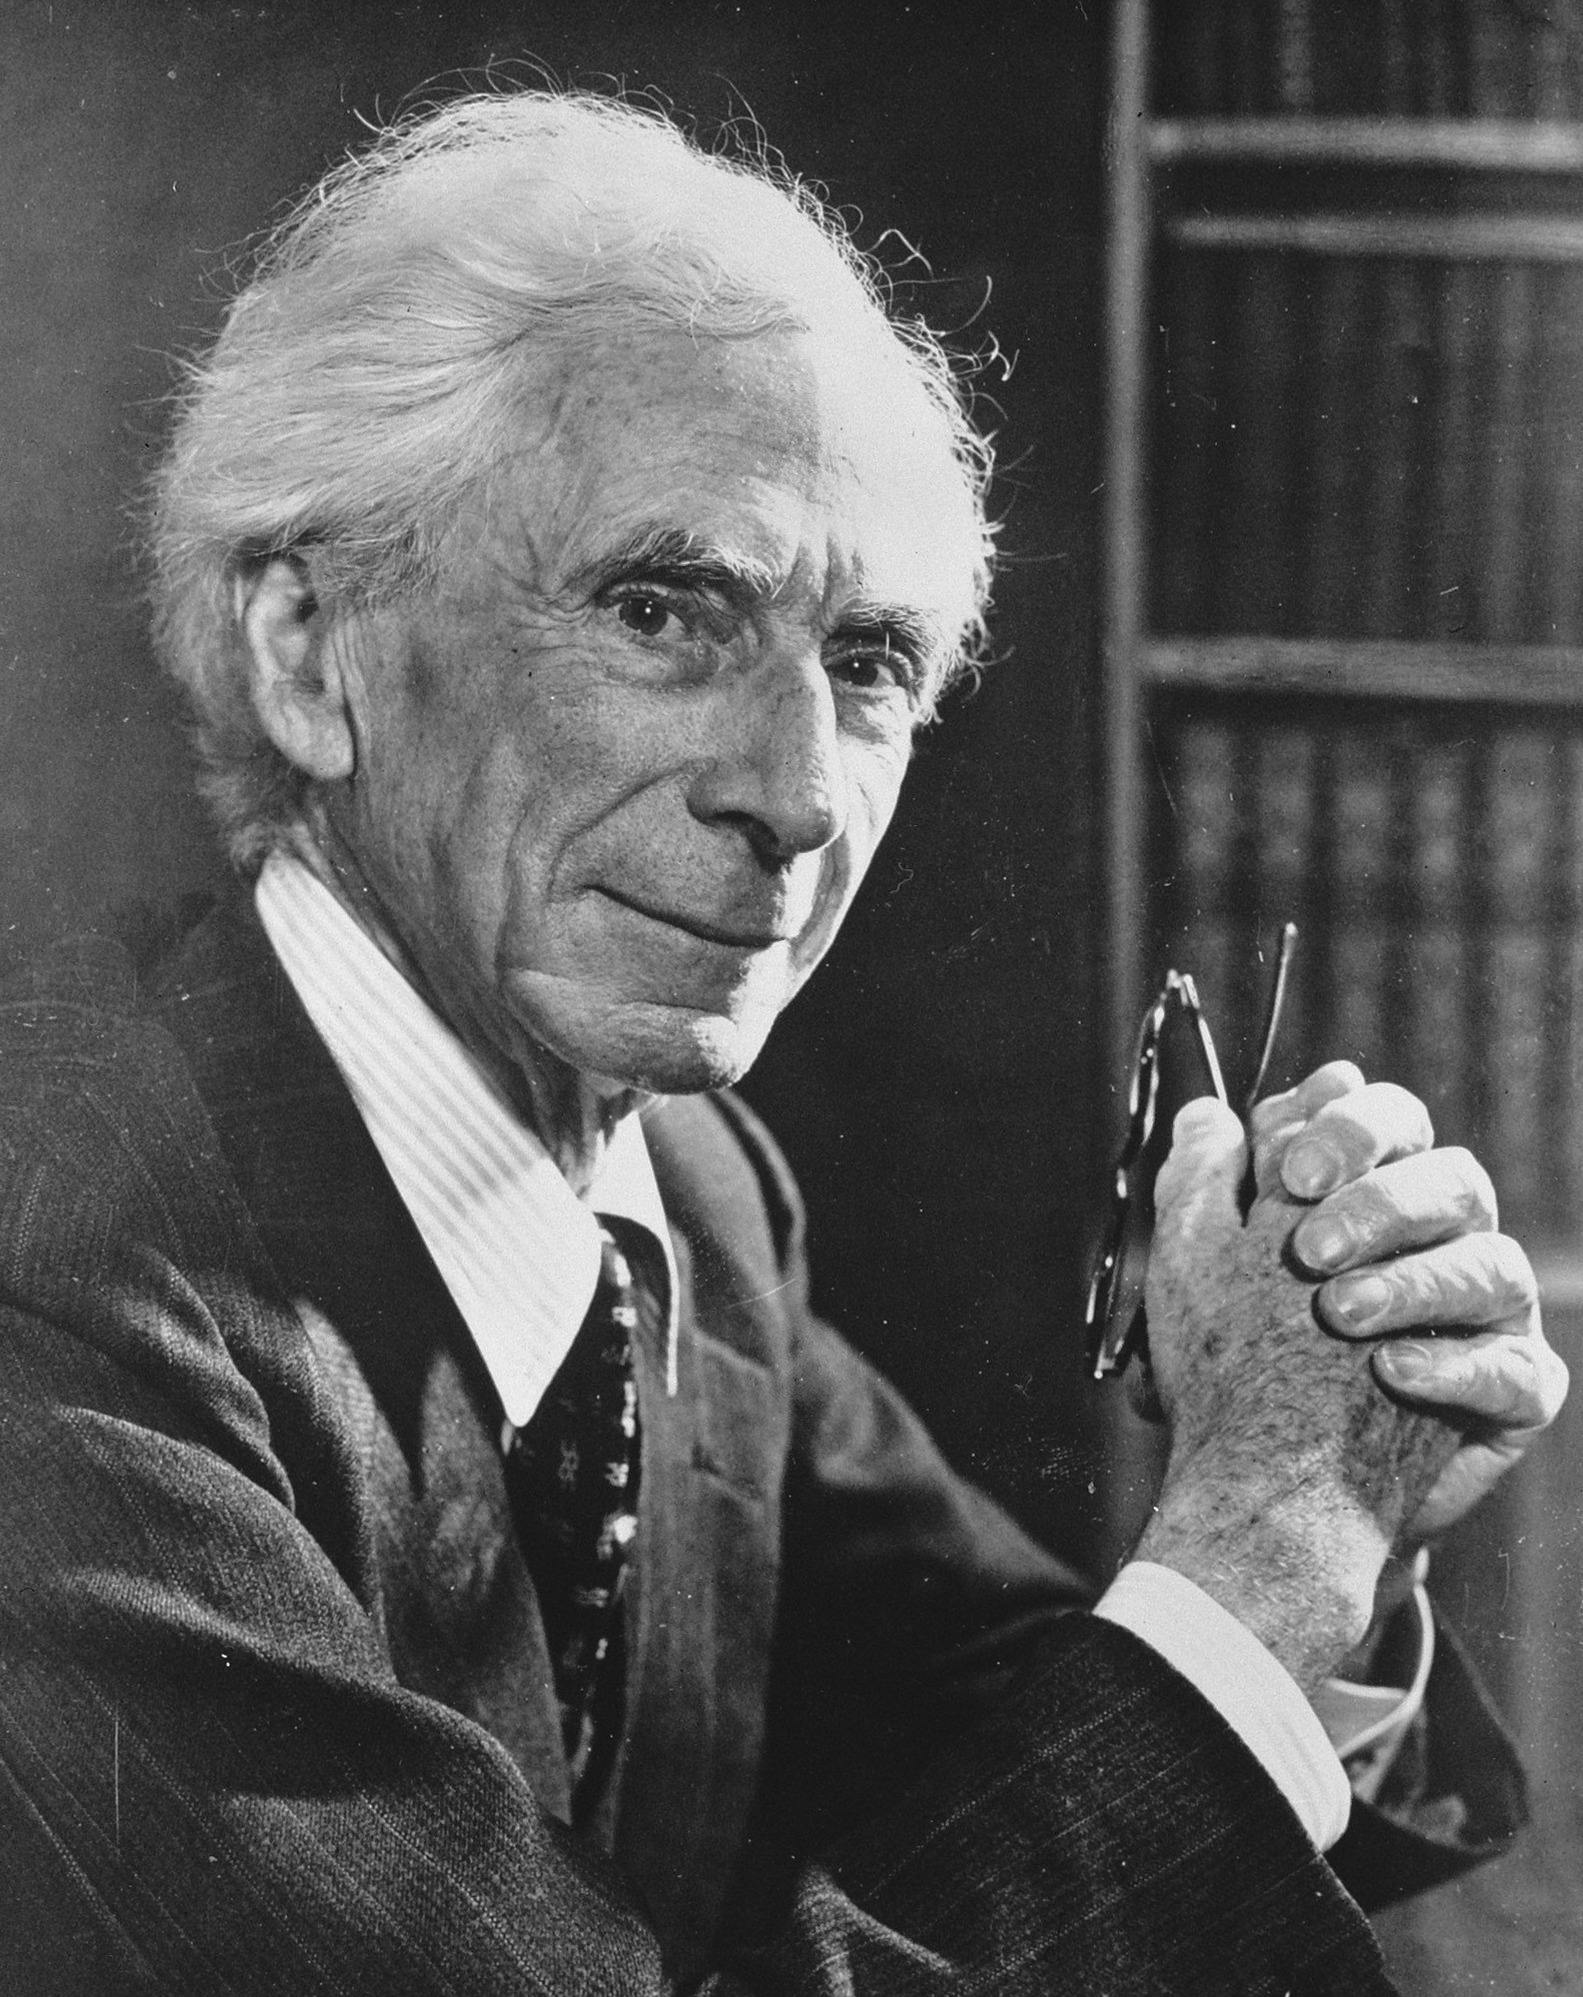
\includegraphics[width=5em]{Bertrand_Russell_1949.jpg}}
  The objects of \(\catcat\) are ``all'' categories. The morphisms are the functors between them.
\end{defn}

The most famous functor among programmers is the \texttt{maybe} functor, also called \texttt{optional}. It lets you bail out of computation early.
\begin{defn}[\texttt{maybe}]
  Let \(\bot\) represent failure. For a type \(A\), \[\texttt{maybe}\,A \define A \cup \bot.\] A function \(f:A \to B\) induces the function that gives up if you pass nothing, otherwise it computes \(f\):
  \[
    \gparen{\texttt{maybe}\, f} x=
    \begin{cases}
      \bot &\text{if } x= \bot \\
      f(x) &\text{if } x\in A
    \end{cases}
  \]
\end{defn}
This is a special case of the \(\texttt{list}\) functor, where the lists are only length \(0\) or \(1\).
\begin{defn}[\texttt{list}]
  \[
    \begin{matrix}
      \texttt{list} :&\text{types} &\to& \text{types} \\
      \obj: &  A &\mapsto & \texttt{list}\, A \\
      \arr:& \paren[\color{gray}\Big]{f:A \to B} &\mapsto & \paren[\color{gray}\Big]{\bracket{x,y,\dots} \mapsto \bracket{f(x), f(y),\dots}}
    \end{matrix}
  \]
\end{defn}

\subsection{Why algebraic topology works}
Algebraic topology is the study of functors from \(\topcat\) to some algebraic category, like \(\ab\) or \(\grp\). Why does this work? The arrows in and out of a topological space tell us about its topology. Hence, the category of topological spaces remembers topological structure. Because functors preserve the categorical structure, clever use of functors out of \(\topcat\) present us this topological structure in a way that's useful.

Confronting \(\topcat\) directly is too hard. \marginnote{Asking if two \(4\)-manifolds have the same fundamental group is already undecidable} There's overwhelmingly many possible continuous functions, and topological structures can be extremely subtle. There's just too much going on in \(\topcat\). Using functors to send spaces to simpler objects, like abelian groups, simplifies the structures while retaining information. And, to the extent arrows in \(\topcat\) capture the structure of spaces (which is fully), functors are the right tool for the job.
\begin{itemize}
  \item Each degree of homology is a functor from topological spaces to abelian groups. \(H_n: \topcat \to \ab\)
  \item The fundamental groupoid is a functor from topological spaces to groupoids.
  \item The fundamental group is a functor from \emph{pointed} topological spaces to groups (you need to pick a base point).
  \item Each degree of \emph{co}homology is a functor  \(H^n:\topcat^{\text{\emph{op}}}\to \ab\)
\end{itemize}
Homology and cohomology in particular seem to hit a sweet spot of retaining enough detail to tell us interesting things, but simplifies enough to be usable.
\subsection{Contravariance}
\begin{defn}[Contravariant functor]
  A contravariant functor is a functor that reverses arrows. Equivalently, a contravaraint functor from \(\cat \to \mathcal{D}\) is an ordinary (covariant) functor \(\cat^{\text{op}} \to \mathcal{D}\)
\end{defn}
These show up all over too.

If you consider two partially ordered sets as categories, contravariant functors are order-reversing (non-increasing) functions.

The powerset is a functor \(\textrm{set}\to\text{ordered}\). Actually, there's two. One's covariant and one's contravariant. They are both familiar. If \(f: A \to B\), then \(f\) acts on a subset \(\alpha \subseteq A\) via \[\alpha \mapsto f(\alpha) \subseteq B.\] This is a covariant functor \cite[243]{natural-equivalence}. On the other hand, \(f\) acts on \(\beta\subseteq B\) via \[\beta \mapsto f^{-1}(\beta) \subseteq A\]
This is going backwards, so it's contravariant \cite[243]{natural-equivalence}.

Both powerset functors undergird point-set topology and measure theory. A function \(f:X\to Y\) is continuous iff \(f^{-1}\) preserves open sets. Analogously, a function is measurable iff \(f^{-1}\) preserves measureable sets. On the other hand, any continuous \(f\) sends compact sets to compact sets, \ie, the induced map on \(2^X\to 2^Y\)  preserves compactness.

Dualizing a vector space, \(\blank^*\), is a contravariant functor:
\[
  \begin{matrix}
    \blank^*:& \veccat &\to& \veccat \\
    \obj:& X & \mapsto &  X^*=\Hom\paren{X,R} \\
    \arr:& \paren[\color{gray}\Big]{f: X \to Y} & \mapsto& \paren[\color{gray}\Big]{f^*: Y^* \to X^*}
  \end{matrix}
\]
where
\[
  f^*(y) = y\circ f : X \to \R.
\]

The cotangent bundle \(T^*\) is a contravariant functor (such an  unfortunate naming \marginnote{I learned functors before manifolds, so the fact that   \(T^*\) is a contravariant functor but contains covariant vectors confused me for weeks}collision) from \(\smooth \to \vecbundle\). A function \(f: M \to N\) induces a function \(f^*: T^*N \to T^*M\).

The hom functors are important in category theory. Every category has them!
\begin{defn}[Covariant hom]
  For an object \(A\in\cat\),
  \[
    \hom(A,\blank)
  \]
  is the covariant hom functor at \(A\). It's defined by
  \[
    \color{darkgray}
    \begin{matrix}
      \hom(A,\blank) :& \cat &\to&\setcat \\
      \obj:& B &\mapsto& \hom(A,B) \\
      \arr:& \paren[\color{gray}\Big]{f:B \to C}& \mapsto& \paren[\color{gray}\Big]{ \black{f\circ \blank} : \hom(A,\black{B}) \to \hom(A,\black{C})}
    \end{matrix}
  \]
  \[
    \begin{tikzcd}
      A
      \ar[-,lightgray!50, shift left= 6pt]{dr}
      \ar[-,lightgray!50, shift left= 3pt]{dr}
      \ar[-,lightgray!50, shift left=-3pt]{dr}
      \ar[dashed]{dr}
      %
      \rar[-,lightgray,shift left=-3pt]{}
      \rar[-,lightgray,shift left= 6pt]{}
      \rar[-,lightgray,shift left= 3pt]{}
      \rar
      %
      & B\dar{f}
      \\
      & C
    \end{tikzcd}
  \]
\end{defn}
\begin{defn}[Contravariant hom]\label{contrahom}
  For an object \(Z\in\cat\),
  \[
    \hom(\blank,Z)
  \]
  is the contravariant hom functor at \(Z\).
  \[
    \color{darkgray}
    \begin{matrix}
      \hom(\blank,Z) :& \cat &\to&\setcat \\
      \obj:& A &\mapsto& \hom(A,Z) \\
      \arr:& \paren[\color{gray}\Big]{f:B \to C}& \mapsto& \paren[\color{gray}\Big]{ \black{\blank\circ f} : \hom(\black C,Z) \to \hom(\black B,Z)}
    \end{matrix}
  \]
  \[
    \begin{tikzcd}
      B
      \ar[-,lightgray!50,shift left= 6pt]{rd}
      \ar[-,lightgray!50,shift left= 3pt]{rd}
      \ar[-,lightgray!50,shift left=-3pt]{rd}
      \ar[dashed]{rd}
      \dar[swap]{f}
      \\
      C
      \rar[-,lightgray,shift left= 3pt]{}
      \rar[-,lightgray,shift left=-3pt]{}
      \rar[-,lightgray,shift left=-6pt]{}
      \rar
      & Z
    \end{tikzcd}
  \]
\end{defn}
Dualizing vector spaces is a special case of \nameref{contrahom}:
\[  \blank^* = \hom(\blank, \R) \]
\section{Natural transformations}
The original motivation of category theory was to pin down what it means for a construction to be \emph{natural}. In the paper \cite{natural-equivalence} that loosed category theory onto the world, Eilenberg \& Mac~Lane open with
\begin{quotation}
  \def\L{L}
  \def\dual{L^{*}}
  \def\ddual{L^{**}}
  \noindent
  ``The subject matter of this paper is best explained by an example, such as that of the relation between a vector space \(\L\) and its `dual' or `conjugate' space \(\dual\)\dots{}Since \(\dual\)  is in its turn a real vector space with the same dimensions as \(\L\), it is clear that \(\L\) and \(\dual\) are isomorphic. But such an isomorphism \emph{cannot be exhibited} until one \emph{chooses} a definite set of basis vectors for \(\L\), and, furthermore the \emph{isomorphism which reults will differ for different choices} of this basis.

  For the iterated conjugate space \(\ddual\), on the other hand, it is well known that one can exhibit an isomorphism between \(\L\) and \(\ddual\) \emph{without using any special basis}
  \marginnote{italics mine, notation changed for consistency}
  in \(\L\). This exhibition of the isomorphism \(\L\cong \ddual\) is `natural' in that is given simultaneously for all finite-dimensional vector spaces \(\L\)'' \cite[231]{natural-equivalence}.
\end{quotation}
This idea of \emph{naturality} is closely related to the idea of \emph{canonicity}, requiring no arbitrary choices. This is a generalization of uniqueness.   Usually, when there's a canonical construction, there's only one thing you can do.

The isomorphism from \(L\) to \(L^{**}\) is canonical in this sense because, with no other information available, there's only one (mod rescaling) nontrivial
\marginnote{The trivial way is \(\_\mapsto 0\).} way to turn an \(x\in L\) into an element of \(L^{**}= \Hom_{\R\text{-linear}}(L^*,\R)\): pass it to \(\phi: L \to \R\).
\[
  \phi \mapsto \phi(x).
\]
There's nothing else you can do because \(x\) and \(\phi\) are totally arbitrary. There's not much all vectors, vector spaces, \& their duals have in common.

The goal of \cite{natural-equivalence}, and, in turn, us, is to capture this. First, for something to be natural, we need \emph{totality}: one construction that works for everything. Second, we need \emph{path-independence}: if the construction is canonical, the specific way you get to it shouldn't matter.

The key insight of \cite{natural-equivalence} is that the correct setting to define naturality is \emph{between functors}.

For the case of \(L \cong L^{**}\), we are looking at two functors: the identity functor, \(1\),
\[
  \begin{matrix}
    1 :& \veccat &\to& \veccat \\
    \obj:& X &\mapsto & X \\
    \arr:& \paren[\color{gray}\Big]{f: X \to Y} &\mapsto & \paren[\color{gray}\Big]{f : X \to Y}
  \end{matrix},
\]
and the double-dual functor, \(\blank^{**}\),
\[
  \begin{matrix}
    \blank^{**} :& \veccat &\to& \veccat \\
    \obj:& X &\mapsto & X^{**} \\
    \arr:& \paren[\color{gray}\Big]{f: X \to Y} &\mapsto & \paren[\color{gray}\Big]{f^{**} : X^{**} \to Y^{**}}
  \end{matrix}.
\]
For a space \(L\), the map \(1\) to \(\blank^{**}\) is
\[
  D_L\define x\mapsto \blank (x) : L \to L^{**}.
\]
Every finite dimensional vector \(L\) space gets its own \(D_L\). We have totality. Drawing only two cases looks like
\[
  \begin{tikzcd}
    X\rar{D_X}\dar[swap]{f}& X^{**}\dar{f^{**}}\\
    Y\rar[swap]{D_Y} & Y^{**}
  \end{tikzcd}
\]
To capture \emph{path-independence}, require the above square commutes:
\[
  D_y \circ f = f^{**} \circ D_x.
\]
In summary,
\begin{defn}[Natural transformation]
  Suppose \(F,G:\cat \to \mathcal{D}\) are two functors.
  A natural transformation \(\tau\) from \(F\) to \(G\),
  \[
    \tau: F \Rightarrow G,
  \]
  is an arrow \(\tau_X\) for each \(x\in\obj(\cat)\) where, for all \(X,Y \in \obj(\cat)\),
  \[
    \begin{tikzcd}
      X \dar[swap]{f}&  F(X)\rar{\tau_X}\dar[swap]{Ff}& G(X)\dar{Gf}\\
      Y        &  F(Y)\rar[swap]{\strut\tau_Y} & G(Y)
    \end{tikzcd}
  \]
  A natural \emph{equivalence}, also called a natural \emph{isomorphism}, is an invertible natural transformation.
\end{defn}

\begin{theorem}
  There is no natural isomorphism \(1 \Rightarrow \blank^*\).
\end{theorem}
\begin{proof}
  First, they go in opposite directions. \(1:\veccat \to \veccat\) is covariant, but
  \(\blank^* : \veccat^{\text{op}} \to \veccat \) is contravariant. We can adapt the naturality condition, but it ends up rather restrictive \cite[234]{natural-equivalence}:
  \begin{equation}
    \begin{tikzcd}
      X\rar[hook, two heads]{\tau_X}\dar[swap]{f} & X^* \\
      Y\rar[hook, two heads,swap]{\tau_Y} & Y^*\uar[swap]{f^*}
    \end{tikzcd}
    \label{contranat}
  \end{equation}
  must commute,
  but this is impossible unless \(f\) is injective, for every \(f\).
\end{proof}
This gives another perspective on \emph{why} orthogonal matrices are invertable. In the category of finite-dimensional \emph{inner} product spaces, whose arrows are orthogonal matrices, there really \emph{is} a natural equivalence \(X\cong X^*\) given by
\[
  x\mapsto \inner{x}{\blank},
\]
so \cref{contranat} does commute! Hence, every arrow in the category must be an injective function. An analogous result works for unitary matrices if you're careful with anti-linearity.

If you're wondering why the naturality square looks familiar,
\begin{defn}[Equivariant map]
  Let \(G\) be a group. Suppose \(A: G \to \Aut(X)\) and \(B: G \to \Aut(Y)\) are group actions (functors). Then an equivariant map is a natural transformation \(f: A \Rightarrow B\):
  \[
    \begin{tikzcd}
      X \dar[swap]{A(g)}\rar{f} & Y\dar{B(g)} \\
      X\rar[swap]{f} & Y
    \end{tikzcd}
  \]
\end{defn}

Natural transformations resemble homotopies between paths. If you think of \(Ff\) and \(Gf\) as paths, then the natural transformation deforms \(F\Rightarrow G\). We can make this insight precise as follows.

\begin{defn}[homotopies \(=\) natural transformations]
  Let \(I=\pi[0,1]\) be the fundamental groupoid of \([0,1]\). It looks like this:
  \[
    \begin{tikzcd}
      0\rar{\eta} & 1
    \end{tikzcd}
  \]
  with the inverse of \(\eta\) and identity arrows omitted. This plays the role of time. Let \(X\) be a topological space. Take two paths
  \[
    f,g : [0,1] \to X.
  \]
  Passing to the fundamental groupoid turns them into functors from \(I\) to \(\pi X\)
  \[
    \begin{tikzcd}
      \text{in }I && \text{in }X \\[-2em]
      && \pi f & \pi g: \\[-1em]
      0\dar{\eta} && f_0 \dar[swap]{\gparen{\pi f} \eta} & g_0\dar{\gparen{\pi g}\eta} \\
      1 && f_1 & g_1
    \end{tikzcd}
  \]
  which send \(0,1\) to endpoints of the curve and send \(\eta\) to the interior of the curve. Then a natural transformation \(\tau\) really is a homotopy between them.
  \begin{align*}
    \begin{tikzpicture}[scale=1.4]
      \draw (-1.3,0);
      \draw[decorate, decoration={coil, aspect=0}] (0,0)--(0,-1);
      \draw[decorate, decoration={coil, aspect=0}] (1,-1)--(1,0);
      \draw (0,-1)--(1,-1) (0,0)--(1,0);
    \end{tikzpicture} \\
    \Downarrow
  \end{align*}
  \[
    \begin{tikzcd}
      0\dar{\eta} && f_0\rar{\tau} \dar[swap]{\gparen{\pi f} \eta} & g_0\dar{\gparen{\pi g}\eta} \\
      1 && f_1\rar{\tau} & g_1
    \end{tikzcd}
  \]
  The requirement the square commutes says you can actually fill in the square. At this level of abstraction, this commutavity is the \emph{only} difference between an honest-to-god homotopy and any four arrows that connect four dots.
  \cite[228]{groupoid}
\end{defn}
In categories that aren't groupoids, natural transformations need not be invertable. In that sense, a natural transformation is a homotopy with an associated direction.

\begin{theorem}
  There is a natural isomorphism between a vector space\eit/ \(V\) and the tangent space\eit/ \(T_a V\) \cite[59]{lee-smooth}. Consider\eit/ \(\veccat_*\), the category of pointed vector spaces. Let\eit/ \(F: \veccat_* \to \veccat\) be the functor that forgets the distinguished point. Let\eit/ \(T_\blank : \veccat_* \to \veccat\) be the tangent space functor. Then the isomorphism
  \[
    \tau_{(V,a)} = \paren{\partial_\blank}_a: V \to T_a V
  \]
  is natural.
\end{theorem}
\begin{proof}
  \[
    \begin{tikzcd}
      (V,a)\dar{L} & V\dar[swap]{L}\rar{\tau_{(V,a)}} & T_a V\dar{dL_a} \\
      (W,La) & W \rar[swap]{\strut\tau_{(W,La)}}& T_{La} W
    \end{tikzcd}
  \]
  Because \(L\) is linear,
  \begin{align*}
    dL_a\paren{\partial_v}_a &= \paren{\partial_{Lv}}_{La} \\
    dL_a \tau_{(V,a)} (v) = dL_a\paren{\partial_v}_a &= \paren{\partial_{Lv}}_{La} = \tau_{\paren{W,La}} Lv
  \end{align*}
  so the diagram commutes.
\end{proof}

Because bundles are often given by functors, their relationships are often natural transformations. For example, for any manifold \(M\) there is an inclusion
\[
  i_M : TM \hookrightarrow T^\otimes M
\]
where \(T^\otimes M = \bigoplus \paren{TM}^{\otimes n}\) is the the tensor-bundle functor. It is natural: the square
\[
  \begin{tikzcd}
    TM\dar[swap]{df} \rar{i_M} & T^\otimes M\dar{df^*} \\
    TN \rar[swap]{\strut i_N} & T^\otimes N
  \end{tikzcd}
\]
commutes because the induced map on tensor bundles agrees with the induced map on tangent bundles.

Because natural transformations go between functors, they're morphisms in some category
\begin{defn}[Functor category]
  Let \(\cat,\dee\) be two categories. Define \(\texttt{functors}(\cat,\dee)\) as the category whose objects are functors \(\cat\to\dee\) and morphisms are natural transformations between them.
\end{defn}
\section{Adjoints}
\begin{defn}[Adjoint]
  The functor \(F: \cat \to \dee\) is a left-adjoint to \(G: \dee \to \cat\), written
  \[
    F \dashv G
  \]
  if
  \[
    \Hom(FX, Y) \cong \Hom(X, GY)
  \]
  and the bijection is natural.
\end{defn}
Consider \(\R\) as an ordered set. Then \(\floor\) and \(\ceil\) are functors \(\R\to \R\) and
\[
  \floor \dashv \ceil
\]
because
\begin{align*}
  \floor x \leq y &\iff x \leq \ceil y\\
  \Hom(\floor x,y) &\phantom{n}\cong\phantom{n} \Hom(x,\ceil y)
\end{align*}

The most famous adjoint pair is the free/forgetful functors.
A free functor from \(\cat \to \dee\) sends an object \(X\in \cat\) to the largest object of \(\dee\) generated by \(X\).

\begin{defn}
  \(\free_\cat\) is defined as the left adjoint to the forgetful functor:
  \[
    \free_\cat \dashv \forget_\cat.
  \]
  Explicitly,
  \[
    \Hom_{\cat}\paren{\free_\cat X, Y} \cong \Hom_{\setcat}\paren{X, \forget_\cat Y}
  \]
  naturally.
\end{defn}
\begin{theorem}
  \[
    \free_\veccat = \Span \qquad{\text{\cite[79]{working}}}.
  \]
\end{theorem}
\begin{proof}
  Suppose \(X = \set{x_i}\). Then
  \[
    \Hom_\cat\paren[\Big]{\grayunderbrace{\free_\veccat \set{x_i}}{?}, Y} \cong \Hom_\setcat\paren[\Big]{\set{x_i}, \forget_\veccat Y}
  \]
  The left-hand side is the set of \emph{linear} functions from the (unknown) \(\free \set{x_i}\). The right-hand side is the set of \emph{all} functions between \(\set{x_i}\to Y\). Using the indexing, an arbitrary function \(f:\set{x_i} \to Y\) is of the form  \(x_i\mapsto f(x_i)= y_i\).

  We want to extend \(\set{x_i}\) to a vector space while extending \(f\) to a linear map \(\overline f: \free X \to Y\). Use \(Y\) as a point of contact between \(f\) and \(\overline f\): identity \(x_i\) with the vector \(\overline{x_i}\) defined by \(\overline f (\overline {x}_i) = y_i\). Therefore, I'll drop the overline on \(\overline{x_i}\). Extend \(\overline f\) by stipulating linearity:
  \begin{equation}
    \label{eq:free-linearity}
    \overline f = \sum_i y_i \otimes x^i = u \mapsto \sum_i y_i x^i(u).
  \end{equation}
  As long as \(\free X\) has no extraneous vectors, \(\overline f\) is uniquely determined by \cref{eq:free-linearity}. In other words,
  \[
    \free X = \Span X.
  \]
  To summarize,
  \[
    \begin{matrix}
      \free:&\setcat &\to&\veccat \\
      \obj:& \set{x_i} &\mapsto& \Span\set{x_i} \\
      \arr:& f & \mapsto & \overline f = \sum f(x_i)\otimes x^i
    \end{matrix}
  \]
  Because \marginnote{You just feel in your heart it's natural}\(\overline f\) is uniquely determined by its values on each \(x_i\), we have naturality in both \(X\) and \(Y\).

  Here's the details.
  Pick an arbitrary \(g \in \Hom_\setcat\paren{\set{x_i}, \set{g(x_i)}}\). By linearity, \(g\) induces
  \[
    \free g: \Span \set{x_i} \to \Span \set{g(x_i)}
  \]
  Because \(\set{x_i}\) is a spanning set, \(\free g\) is completely determined. Therefore,
  \[
    \begin{tikzcd}
      \Hom\limits_\veccat \paren{\free \set{x_i}, Y} \dar[swap]{\free g}\rar[<->]{\overline{\blank}} & \Hom\limits_\setcat \paren{\set{x_i}, \forget Y}\dar{g} \\
      \Hom\limits_\veccat \paren{\free \set{g(x_i)}, Y}\rar[<->]{\overline{\blank}} & \Hom\limits_\setcat \paren{\set{g(x_i)}, \forget Y}
    \end{tikzcd}
  \]
  commutes. The equivalence is natural in \(X\).

  On the other hand, suppose \(h \in \Hom\limits_\veccat\paren{Y, h(Y)}\). Then
  \[
    \begin{tikzcd}
      \Hom\limits_\veccat \paren{\free \set{x_i}, Y} \dar[swap]{h\circ\blank}\rar[<->]{\overline\blank} & \Hom\limits_\setcat \paren{\set{x_i}, \forget Y}\dar{\gparen{\forget h}\circ\blank} \\
      \Hom\limits_\veccat \paren{\free \set{x_i}, h(Y)} \rar[<->]{\overline\blank} & \Hom\limits_\setcat \paren{\set{x_i}, \forget h(Y)}
    \end{tikzcd}
  \]
  Suppose \(f:\set{x_i}\to Y\). Along either route, you get a map that sends \(x_i \mapsto h\circ f(x_i)\). Because this uniquely determines the induced linear map,
  \[
    \overline{h\circ f} = h\circ \overline f,
  \]
  and the diagram commutes.
\end{proof}
\subsection{Internal homs and tensors}
Usually hom-sets have additional structure. Sometimes, they're even objects in the same category. For example, in \(\setcat\), hom-sets are sets, hence objects. In \(\veccat\), pointwise addition \& multiplication make
\[
  \Hom_\veccat(X,Y)
\]
into a vector space. It's even finite-dimensional when both \(X\) and \(Y\) are. In \(\topcat\),
\[
  \hom_\topcat(X,Y) \subseteq X^Y
\]
and \(X^Y\) has the product topology. Then \(\hom_\topcat(X,Y)\) inherits the subset topology, the topology of pointwise convergence.

\begin{defn}[in/external hom]
  In these cases, it's useful to distinguish between the \emph{external} homs, the set of functions, and the \emph{internal} homs, the object in the category. Denote the \emph{internal} hom as
  \[
    \bracket{X,Y} \in\obj(\cat) \quad\text{where } X,Y\in \obj(\cat)
  \]

  A category with internal homs is called \emph{closed}.
\end{defn}

With internal homs, we can now have arrows into hom-sets. Consider \(\veccat\).
\[
  \begin{tikzcd}
    A \rar{f}& \bracket{B,C}
  \end{tikzcd}
\]
Choosing an \(a\in A\) gives
\[
  \begin{tikzcd}
    B \rar{f(a)} & C
  \end{tikzcd}
\]
Sometimes I draw this like
\[
  \begin{tikzcd}
    A \rar{f} & \Big\lbrack B
    \rar[shift left=8pt]
    \rar[shift left=4pt]
    \rar
    \rar[shift left=-8pt]
    \rar[shift left=-4pt]
    & C \Big\rbrack
  \end{tikzcd}
\]
but I've never seen that anywhere else.

The map
\[
  (a,b) \mapsto f(a)(b)
\]
is bilinear:
\[
  \paren{f(a+t\alpha)}b =  \paren{f(a) + t f(\alpha)}b = f(a)(b) + t f(\alpha)(b)
\]
and
\[
  f(a)(b+t\beta) = f(a)(b)+tf(a)(\beta)
\]

Internal homs give us one way to define multilinear maps from linear maps. The other way is with the tensor product. A bilinear map can be written
\[
  f : A \otimes B \to C
\]
or
\[
  f: A \to \bracket{B,C}.
\]
In other words, there's a natural equivalence
\[
  \bracket{A\otimes B, C} \cong \bracket{A, \bracket{B,C}}
\]
\ie, they're adjoints:
\begin{defn}[Tensor-hom adjunction]\label{tensor-hom-adj}
  The tensor-hom adjunction is
  \[
    \blank \otimes  B\dashv \bracket{B,\blank}
  \]
  It holds in \(\veccat\) for example.
\end{defn}
In categories with both a tensor product and internal homs, \namecref{tensor-hom-adj} is usually satisfied. In categories with internal homs only, it suggests an approach to define a tensor product.

In \(\setcat\), the tensor product (in this sense) is just the cartesian product. In \(\setcat\),
\[
  [Y,Z] = Z^Y.
\]
Then
\[
  [X,[Y,Z]] = \paren{Z^Y}^X \cong \paren{Z^{X\times Y}} = [X\times Y, Z].
\]
The \setcat-isomorphism (bijection) is natural and given by Currying, \ie, send \(f\in [X,[Y,Z]]\)
\[
  (x,y) \mapsto f(x)(y)
\]


\section{Sheaves}
\marginnote{This doesn't really belong here, but it's here anyway.}
Before defining sheaves, I'll explain why geometers working in \(\smooth\) don't need them. In \(\smooth\), we have smooth bump functions, smooth cutoff functions, and smooth partitions of unity. Therefore, we can extend local constructions globally.

Suppose \(f:U \to \R\) for \(U\subseteq M\). If \(\phi\) is a bump function on \(U\) and \(\phi(V)=1\) for some \(V\subset U\).  Then
\[
  \paren{\phi f}(x) =
  \begin{cases}
    f(x) &\text{if } x\in V \\
    0 &\text{if } x\notin U.
  \end{cases}
\]
It contains essentially the same data as \(f\), but it's defined on all of \(M\). In \(\smooth\), we can be sloppy with domains.

This is not true anymore for analytic functions. Analytic functions are rigid. Take \(f(x)=e^x\) for example. Just from its values on the infinitesimal neighborhood \([-\epsilon,\epsilon]\), we can already get its Taylor series:
\[
  f^{(n+1)} = \lim_{h\to 0} \frac{f^{(n)}(h)-f^{(n)}(0)}{h} = 1
\]
fits entirely within \([-\epsilon,\epsilon]\). But now
\[
  f(x) = \sum \frac{f^{(n)}(0) x^n}{n!}  =e^x
\]
converges on all of \(\complex\). Its values on an \emph{infinitesimal} neighborhood fix the values \emph{everywhere} in \(\complex\).

The case \(e^x\) is an ideal one, \(e^x\) is entire, but the point stands in general:
\begin{theorem}[Liouville]
  Every holomorphic function \(\complex\to\complex\) is either constant or unbounded \cite{wiki-liouville}.
\end{theorem}
This eliminates the hope of analytic bump functions.
Similarly, there's
\begin{theorem}[Maximum modulus principle]
  A holomorphic function\eit/ \(U \to \complex\) is either unbounded or locally constant \cite{wiki-max-mod}.
\end{theorem}
and the especially frustrating
\begin{cor}
  ``Any holomorphic function on a compact Riemann surface is necessarily constant'' \cite{wiki-liouville}.
\end{cor}

The situation is even worse when we look at polynomials and rational functions. A polynomial can't have more zeroes than its degree, so any polynomial that's zero infinitely often is zero constantly. Additionally, rational functions are interesting, but they have poles ({\footnotesize\texttt{s/rational/meromorphic}}). Sometimes the poles are the interesting part. If we want to study rational functions as \emph{functions} instead of formal symbolic expressions, we are forced to be cautious with their domains.

For example, the only rational functions defined on all of \(\complex\) are plain-old polynomials ({\footnotesize \texttt{s/rational/meromorphic,} \texttt{s/polynomial/holomorphic}}). The only rational functions defined on \(\complex-\set{0}\) are
\[
  \set{\frac{p(x)}{x^n} : n \in \N, p \text{ is a polynomial}}.
\]
On \(\complex-\set{a,b}\), the only rational functions are
\[
  \set{\frac{p(x)}{(x-a)^m(x-b)^n}}
\]
Shrinking the domain grows the set of functions, which is backwards from \(\setcat\).

To organize the situation, organize the relationships between the functions defined on various open sets. Additionally, we want to ensure the copy of \(f(x)\) defined on the set \(U\) and the copy defined on \(V\) really are the same thing. Enter sheaves.

Well, first, presheaves
\begin{defn}[Category of opens]\marginnote{\ie, draw one arrow \(A\to B\) iff \(A\subseteq B\).}
  Let \(\tau\) be the category of open sets on your space ordered by \(\subseteq\).
\end{defn}
\begin{defn}[Presheaves]
  A presheaf is a functor \(F: \tau^\op\to \setcat\).
\end{defn}
The arrows in \(\tau^\op\) are reverse-inclusions, also called \emph{restrictions}. When you restrict from a bigger set to a smaller one, the presheaf follows suit.
\begin{itemize}
  \item The identity functor is a presheaf, trivially.
  \item \(C^\infty:\tau^\op \to \setcat\) is a presheaf on a smooth manifold. Each open set \(U\) gets its set of functions \(C^\infty(U)\). Restrictions are the usual restrictions of a function's domain.

  \item \(\rat: \tau^\op \to \setcat\) is a presheaf on \(\complex\). Each open set gets its set of rational functions. Restrictions are still usual restriction of domain, but something interesting happens: restrictions \emph{are not} surjective. \(\rat(\complex)\) are just polynomials, but \(\rat(\complex - \Z)\) are every rational function with singularites on \(\Z\). Additionally, because polynomials, hence rational functions, are fully determined by their values on finitely many points, restrictions \emph{are} injective.
\end{itemize}

We're not quite there, though. We want to make sure, in some sense, functions are the same entity after restriction. Wikipedia calls elements in the sheaf sections \cite{wiki-sheaf}, which I don't love. But I'm not gonna call it wheat fields, so section it is.
\begin{defn}[Sheaf]
  \def\S{\mathcal S}
  A sheaf is a presheaf \(\S:\tau^{\op}\to \setcat\) satisfying locality and gluing. Let \(U\) be an open set, covered by \(U_i\),
  \[
    U= \bigcup U_i.
  \]
  \begin{itemize}
    \item Locality. Sections on \(U\), aka elements in \(\S(U)\), are completely determined by their values locally. Two sections are the same if they're the same locally everywhere, \ie, on each \(U_i\). Suppose \(s,t\in \S(U)\). Then locality says
          \[
          \gparen{\forall i \quad s|_{U_i} = t|_{U_i} } \implies s = t
          \]

    \item Gluing. If a collection of sections agree on overlaps, you can glue them together. Suppose there is a family \(s_i\in \S(U_i)\) that agrees on overlaps,
          \[
          \forall i,j \quad { s_i|_{U_i \cap U_j} = s_j|_{U_i\cap U_j} }
          \]
          then there is an \(s\in \S(U)\) formed by gluing them together:
          \[
          s_i = S|_{U_i}
          \]
  \end{itemize}
  \cite{wiki-sheaf}
\end{defn}
Most things on manifolds are sheaves. \(C^\infty\) is a sheaf, but so are the space of vector fields, tensor fields, and differential forms. You can restrict them, they're fully defined by their local behavior, and you can glue them when they agree. In \(\smooth\), this machinery can be overkill, but when you lose partitions of unity, it's crucial.

\section{Algebra}
\revmarginnote{This \emph{really} doesn't belong here.}
The most important kinds of algebraic spaces roughly mirror the way we teach kids numbers, which makes a good mnemonic
\begin{itemize}
  \item monoids \(\sim (\N,+)\) \marginnote{You don't see monoids in abstract algebra 1, but they're all over category theory}\\
        There's a binary operation (\(+\)) and an identity element (\(0\))
  \item groups \(\sim (\Z,+)\) integers \\
        Now inverses (negatives)
  \item rings \(\sim (\Z,+,\times)\) \\
        Now there's multiplication. It distributes over addition
  \item fields \(\sim (\Q,+,\times)\)\marginnote{in fields, multiplication \emph{does} need to commute} \\
        And fractions!
\end{itemize}
Addition in rings is commutative. Some authors require multiplication in rings be commutative, but some do not because then \(n\times n\) matrices are a ring. Either way, this is a good example to keep in mind, because square matrices show you lots of ways multiplication can fail to be invertable.

\begin{defn}[ring]
  A ring \((R,+,\cdot,0,1)\) is
  \begin{itemize}
    \item An abelian group under \((+,0)\) \marginnote{using group and monoid in the definition lets us omit writing all the associativity laws.}
    \item A monoid under \((\cdot,1)\)
    \item And distributive:
          \begin{align*}
            a(b+c)\phantom{c} &= ab + ac. \\
            (a+b)c &= ac + bc
          \end{align*}
  \end{itemize}
\end{defn}
Sometimes people drop the requirement that \(1\), a multiplicative identity, exists. Sometimes this is called a rng, a ring without \emph{i}dentity. Similarly, sometimes people drop the requirement additive inverses exist and call it a rig, a ring without \emph{n}egatives. I propose the term \emph{rin}, a ring without \emph{g}ommutativity. In other words, I'm assuming rings commute.

\begin{defn}[Polynomial ring]
  Given a ring \(R\), the polynomials with coefficients in \(\R\) and formal variable \(x\), written
  \[
    R[x],
  \]
  is a ring.

  Similarly, \(R[x,y,z]\) is the ring of polynomials in all three variables.
\end{defn}

\begin{defn}
  The tensor algebra \(V^\otimes\) of a vector space \(V\) is a ring.
\end{defn}

You can't quotient by any old group, only \emph{normal} subgroups. Analogously, you can't quotient by any subrng, only \emph{ideals}.
Recall
\[
  0 + 0 = 0
\]
so \(0\) is closed under addition,
and
\[
  0x = 0,
\]
\(0\) is absorbative under multiplication. Any set that can be collapsed to zero must have these properties as well

\begin{defn}[Ideal]
  A subset \(I\subseteq R\) is an ideal iff \marginnote{In a \emph{rin}, you have to distinguish left-ideals from right-ideals, so I'm skipping them (I'm committed to the bit).}
  \begin{itemize}
    \item \(I\) is closed under addition, \ie
          \[
          \forall x,y\in I\quad x+y \in I
          \]
          or, more concisely, \(I+I=I\).
    \item \(I\) is absorbative under multiplication, \ie
          \[
          \color{darkgray}
          \forall r\in \black R\  \forall x \in I\quad  rx \in I
          \]
          or, more concisely, \(RI=I\).
  \end{itemize}

  The ideal generated by \(x\) is written \(\paren x\).
\end{defn}

This is already enough to do something interesting:
\begin{defn}[Dual numbers]
  The dual numbers are
  \[
    \R[x]/\paren{x^2}
  \]
\end{defn}
Dual numbers contain nilpotent elements. After taking quotients, \(x^2=0\). As a consequence, \(x\) is non-invertable.

\begin{defn}[Complex numbers]
  \[
    \complex = \R[x]/\paren{x^2+1}
  \]
\end{defn}
Interestingly, \(\complex\) is a field: every nonzero complex number is invertable, even though the definition looks almost the same as dual numbers.  The reason for this is \(x^2+1\) is an \emph{irreducible} polynomial over \(\R\). We see the same thing happen in \(\Z/\paren 4\) vs \(\Z/\paren{5}\).  In \(\Z/\paren 4\), \(2^2=4\equiv 0 \pmod 4\), but every nonzero element is invertable in \(\Z/\paren 5\) because \(5\) is prime.

\begin{defn}[Hyperbolic numbers]
  \[
    \R[x]/\paren{x^2-1}
  \]
\end{defn}
Because \(x^2-1= (x+1)(x-1)\), this isn't a field. In fact, after taking mods, we get
\[
  (x+1)(x-1) = 0.
\]

\begin{defn}
  \[
    \Q[\sqrt 2] = \Q[x]/\paren{x^2-2}
  \]
\end{defn}
Because \(x^2-2\) is irreducible over \(\Q\), we get a field again.

\begin{theorem}
  In \(\Q\), every ideal trivial---either\eit/ \(\set{0}\) or\eit/ \(\{\Q\}\).
\end{theorem}
\begin{proof}
  Suppose \(I\) is an ideal. If \(I=\set 0\), we're done. Otherwise, there is some \(x\in I\) such that \(x\neq 0\). But then \(x^{-1}\in \Q\) exists. By hypothesis \(I\) is absorbative, so
  \[
    Ix^{-1} =I
  \]
  But then \(xx^{-1}=1\in I\). Applying absorbativity again, \(y=y1 \in yI = I\) for any \(y\in \Q\). Hence \(I=\Q\).
\end{proof}
Actually, this proof generalizes.
Ideals measure the failure of a ring to be a field.
\begin{theorem}
  A ring \(R\) is a field iff its only ideals are \(R\) and \(0\).
\end{theorem}
\begin{proof}
  \begin{itemize}
    \item If ring, the only ideals are \(0\) and \(R\).\\
          Take an ideal \(I\neq 0\). Pick a nonzero \(x\in I\). If \(x\) has an inverse, then by absorbativity
          \[
          xx^{-1} = 1 \in I.
          \]
          But then, by absorbativity, \(I=R\).
    \item If the only ideals are \(R\) and \(0\), it's a ring.  \\
          Pick a nonzero \(x\in R\). Then \(\paren{x}\), the set of multiples of \(x\), is an ideal. By hypothesis, it contains \(1\). Therefore, there is some \(y\) such that
          \[
          xy =1.
          \]
  \end{itemize}
\end{proof}

Ideals generalize the idea of multiples of a number:
\begin{theorem}\marginnote{ideals like \(\paren{a}\) are called \emph{principal}}
  Every ideal in \(\Z\) is of the form \(\paren{a}\), the set of multiples of \(a\).
\end{theorem}
\begin{proof}
  Suppose \(I\) is an ideal in \(\Z\). If \(I=\set 0\), then \(I=\paren{0}\), so we're done.

  Suppose \(I\neq 0\). Let \(a\) be the smallest positive element of \(I\). Let \(b>a\) be an element of \(I\). By repeated subtraction (Euclid's algorithm), find \(\texttt{gcd}\paren{a,b}\). Because \(I\) is closed under subtraction, \(\texttt{gcd}\paren{a,b}\in I\). By construction,
  \[
    \texttt{gcd}\paren{a,b} \leq a
  \]
  But by assumption \(a\) is minimal,
  \[
    a\leq\texttt{gcd}(a,b)
  \]
  so \(a=\texttt{gcd}(a,b)\). Then \(b\) is a multiple of \(a\).

  By negating everything, the same argument applies to the negative side of \(I\). Conclude
  \[
    I = \paren{a},
  \]
  the ideal generated by \(a\).
\end{proof}
In ``easy'' rings, ideals are just multiples\marginnote{In a \emph{principal ideal domain}, every ideal is principal.}. If a ring has a \(\texttt{gcd}\) algorithm, then ideals are of this form.  Unfortunately, life is not so simple.

\begin{theorem}
  \(\complex[x,y]\) has an ideal that's not merely a set of all multiples. It's given by
  \[
    \paren{x,y}
  \]
\end{theorem}
\begin{proof}
  Consider
  \[
    \paren{x,y} = \set[\big]{\text{polynomials with \(0\) constant term}}.
  \]
  Certainly, we can quotient by \(\paren{x,y}\), in effect, setting \(x=y=0\).

  However, there is no \(\texttt{gcd}(x,y)\) because both \(x\) and \(y\) are indeterminate, hence irreducible.
\end{proof}
\begin{theorem}[Unique factorization fails]
  Unique factorization fails in \[\Z\bracket{\sqrt{-5}}.\] There are two distinct irreducible\marginnote{irreducible \(\neq\) prime, but never mind. They're the same in \(\Z\), but not everywhere.} factorizations of\eit/ \(6\),
  \[
     \gparen{1 + \sqrt{-5}}\gparen{1-\sqrt{-5}} =6= \gparen 2\gparen 3.
  \]
\end{theorem}
\begin{proof}
  The trick is to use the norm
  \[
    N\gparen{a+b\sqrt{-5}} \define \gparen{a+b\sqrt{-5}}\gparen{a-b\sqrt{-5}} = a^2 + 5 b^2.
  \]
  It's multiplicative,
  \[
    N(xy) = N(x)N(y),
  \]
  so a necessary condition for \(x\) divides \(z\) is \(N(x)\) divides \(N(z)\). This screens out possible factors, so we can check irreducibility.
  \begin{itemize}
    \item \(2\) is irreducible.\\ Suppose \(xy=2\). Then
          \[
          N(x)N(y) = N(2)= 4 = 1\cdot 4 = 2\cdot 2.
          \]
          Without loss of generality, either \(N(x)=1\) or \(N(x)=2\). Write \(x = a + b\sqrt{-5}\). Suppose
          \begin{equation}
            \label{unique-factor-fail-n=1}
            N(x)= a^2+ 5b^2 = 1 \implies a = \pm 1, b=0.
          \end{equation}
          so \(x=\pm 1\). Alternately, suppose
          \[
          N(x)=a^2+5b^2=2 \implies a^2= 2\implies \text{no solution over \(\Z\)}
          \]
    \item  \(3\) is irreducible.\\ By the same argument,
          \[
          N(3) = 9 = 1 \cdot 9 = 3 \cdot 3
          \]
          so either \(N(x)=1\) or \(N(x)=3\). From \cref{unique-factor-fail-n=1}, we know the only solution for \(N(x)=1\) is \(x=\pm1\). So consider \(N(x)=3\):
          \[
          N(x)=a^2+5b^2 = 3 \implies{a^2=3} \implies \text{no solution over \(\Z\)}
          \]
    \item \(1+\sqrt{-5}\) is irreducible.
          \[
          N\gparen{1+\sqrt{-5}} = 1+5 = 6= 1\cdot 6 = 2\cdot 3
          \]
          So if \(xy=6\), then either \(N(x)=1\) or \(N(x)=2\). But we already checked the only solution is \(x=\pm 1\).
    \item \(1-\sqrt{-5}\) is irreducible.
          \[
          N\gparen{1-\sqrt{-5}} = 1 + 5  = 6 = 1\cdot 6 =2 \cdot 3,
          \]
          so the same argument works.
  \end{itemize}
\end{proof}
Algebraists, unwilling to give up unique factorization, defined maximal and prime ideals.
\begin{defn}[Maximal ideal]
  An ideal \(I\) over ring \(R\) is maximal if the only bigger ideal is all of \(R\).
\end{defn}
In \(\Z\), maximal ideals are exactly \(\paren p\) when \(p\) is prime.

An analogous result holds in \(\complex[x]\). Because of \revmarginnote{the fundamental theorem is necessary. This only works for polynomials over \emph{algebraically complete} fields}the fundamental theorem of algebra, every polynomial splits into linear factors, uniquely. Thus, the maximal ideals are exactly \(\paren{x-a}\).

Every maximal ideal is also prime:
\begin{defn}[Prime ideal]
  %\marginnote{For a prime number,\\\,\\ \(p\divides ab\) \(\implies\)\\ \(p\divides a\) or \(p\divides b\)\\\,\\ (the \(\divides\) means divides)}
  An ideal \(P\) is prime iff
  \[
    P \ni ab \implies P\ni a \text{ or } P \ni b
  \]
  in analogy with the fact\marginnote{``\(\divides\)'' means divides}
  \[
    p \divides ab \implies p\divides a \text{ or } p \divides b
  \]
  for \(p\) a prime integer.
\end{defn}
Prime ideals need not be maximal.
In fact, the minimal (zero) ideal is often prime
\begin{lemma}\marginnote{\(\Z/\paren 4\) has zero-divisors: \(2^2=0\). \\[1ex]Dual numbers have zero-divisors, \(\epsilon^2=0\).}
  In a ring with no zero-divisors, the ideal \(\paren 0\) is prime. \revmarginnote{The converse is true too.}
\end{lemma}
\begin{proof}
  If \(R\) has no zero-divisors, then \(0=ab\) only if \(a=0\) or \(b=0\). Suppose
  \[
    \paren 0 \ni ab.
  \]
  Because \(\paren 0 = \set{0}\), conclude \(0=ab\). By hypothesis, either \(a=0\) or \(b=0\). Suppose \(a=0\). Then
  \[
    \paren{0}\ni a.
  \]
  By the same argument, if \(b=0\) then \(\paren 0 \ni b\).
\end{proof}
The prime ideals of \(\Z\) are the maximal ideals \emph{and} \(\paren 0\). This is typical of ``easy'' rings. When you have a \texttt{gcd} algorithm, every maximal ideal is generated by an irreducible element, and the prime ideals are maximal or \(\paren 0\).

\subsection{Algebraic geometry}
In algebraic algebraic geometry, ideals are systems of equations, more or less. Consider the ring of polynomials
\[
  \complex[x,y,z].
\]
Any system of polynomial equations generates an ideal. For example,
\[
  \left.
  \begin{matrix}
    x = z^2 \\
    y = 3z
  \end{matrix}\
  \color{gray}\right\}
  \implies
  \color{black}
  \paren{x-z^2, y-3z}
\]
Quotienting out by this ideal amounts to setting
\[
  \begin{matrix}
    x-z^2 = 0 \\
    y-3z = 0
  \end{matrix}
\]
The basic manipulations to solve or simplify systems of equations, like Gaussian elimination, stay within the ideal. For example, squaring \(y=3z\) translates to multiplying \(y-3z\) by \(y+3z\):
\[
  \paren{y-3z}\paren{y+3z} = y^2-9z^2
\]
so that, too, is in the ideal. Continuing down that road will reveal
\[
  9x - y^2 \in \paren{x-z^2, y-3z}
\]

You can encode points in the base space as systems of equations, hence ideals. The point \((a,b,c)\) becomes the system \(x=a,y=b,z=c\) becomes the ideal
\[
  \paren{x-a,y-b,z-c}.
\]
This observation will become \nameref{nullenstellensatz}.

This classical result about polynomial division tells us a lot about ideals in \(\complex[x]\):
\begin{theorem}[Remainder-root theorem]
  Suppose \(p(x)\) is a polynomial. Then
  \[
    p(x) \equiv p(a) \pmod {x-a}.
  \]
  Explicitly,
  \[
    p(x) = q(x)\paren{x-a} + p(a).
  \]
\end{theorem}
Polynomial evaluation is a special case of quotienting by ideals. This characterizes the ideals generated by linear factors:
\[
  \paren{x-a} = \set[\big]{p(x) : p(a)=0}.
\]

\begin{theorem}[Hilbert's Weak Nullenstellensatz]\label{nullenstellensatz}
  The maximal ideals of
  \[
    \complex[x_1,\dots x_n]
  \]
  are exactly
  \[
    \paren{x_1-a_1,\dots x_n-a_n} \hbox to0pt {\qquad
  \text{\cite[107]{rising-sea2024}.}}
  \]
\end{theorem}
\marginnote{\cite[56]{real+functional} has an analogous theorem for ideals of continuous functions.  It needs convergence. (Algebraists doing analysis)}
If we think of polynomials as \emph{functions} over the space \(\complex^n\), taking maximal ideals brings us back to the base space. Taking quotients by maximal ideals \emph{evaluates} the function at the corresponding point.

This hints at a \emph{geometric} interpretation of ideals. Suppose \(I\) is an ideal, not maximal, over \(\complex[x_1\dots x_n]\). Then \(I\) can be refined to some maximal ideal:
\[
  I\subseteq (x_1-a_1,\dots x_n-a_n).
\]
Geometrically, this means the subset of \(\complex^n\) associated to \(I\) contains the point \((a_1,\dots a_n)\).

What about solution sets of systems of equations? Consider the solution set of \(y=x^2\) over \(\complex^2\). But instead of carving the solution out of the complex plane, use ideals in \(\complex[x,y]\):
\[
  \complex[x,y]/\paren{y-x^2}
\]
What does this quotient look like? It just sets \(y=x^2\)
\[
  p(x,y) \mapsto p(x,x^2) : \complex[x,y] \to \complex[x]
\]
We've restricted the functions in \(\complex[x,y]\) to \(y=x^2\) by taking this quotient.

What are the maximal ideals containing \(\paren[]{y-x^2}\)? The points on the parabola! For example, if \(a\in\complex\), the point \((a,a^2)\) lies on the parabola, and the ideal
\[
  \paren{x-a,y-a^2} \supseteq \paren{y-x^2}
\]
\begin{proof}
  Here's the details. To be in the ideal, \(y-x^2\)   must be a linear combination of \(x-a\) and \(y-a^2\). You can start squaring and solving, but ordinary polynomial division with remainder does the trick. \marginnote{Because the division algorithm only works for one variable at a time, treat \(y\) as a constant.}
  % or monovariate polynomials?
  \[
    \begin{matrix}
      \color{darkgray}
      &    & x  & +a    \\
      \hline\rule{0pt}{\normalbaselineskip}
      x-a\Big) &  x^2 & & &-y      \\
          &x^2  &- ax \\
      \hline
          &     & ax & \\
          &     & ax & - {a^2} \\
      \hline
          &     &    & \black{a^2}& -y\rule{0pt}{\normalbaselineskip}
    \end{matrix}
  \]
  so the remainder is \(-y+a^2\) and, all together,
  \[
    -y+x^2 = \paren{x-a}\paren{x+a} - (y-a^2) \in \paren{x-a,y-a^2}
  \]
\end{proof}
\section{Reading list}
\begin{itemize}
  \item Eilenberg \& Mac Lane \book{Categories for the working mathematician} \cite{working} is the canonical reference for category theory. They are founders. But the book is hard.
  \item The Catsters have a series of short youtube lectures on category theory. That's where I learned universal properties \url{https://www.youtube.com/user/TheCatsters/}.
  \item Baez \& Stay ``Physics, topology, logic and computation: a Rosetta stone'' \cite{rosetta} looks at correspondences in categories, particularly monoidal categories and braidings, of interest in all these subjects.

  \item Brown's \book{Topology and Groupoids} \cite{groupoid}. If you want to learn category theory through the fundamental groupoid, read chapter 6.

  \item Aluffi's \book{Algebra Chapter 0} is an introduction to algebra with category theory (category theory is traditionally a grad-school topic).

  \item Dummit \& Foote \cite{dummit+foote} covers a ton of undergrad algebra, but no category theory.

  \item Vakil's \book{Rising Sea} is an introduction to the machinery of modern algebraic geometry. From what I've read so far, its  writing's clear and stresses intuition.

  \item Lang's \book{Algebra}. I brought up a Lang book to a professor once, who said  ``he's' a fallen Bourbaki-ist''. Not a good first algebra book, but it has a lot of info, generality, and a sense of taste, if not too Bourbaki.

\end{itemize}
\printbibliography
\end{document}
